%% ============================================================================
%% Chapter 4: Data on the Wire -- Serialization Formats & Data Contracts
%% Mastering APIs: From Zero to Production Guru
%% ============================================================================
\chapter{Data on the Wire: Serialization Formats \& Data Contracts}
\label{ch:serialization}

%% ----------------------------------------------------------------------------
%% Executive Summary
%% ----------------------------------------------------------------------------
Every API call is, at its core, an act of translation. Inside your process, a
\emph{Part} is a graph of objects living in heap memory; on the wire it must become
an ordered sequence of bytes; on the far side it must be reconstructed into an
equivalent structure without loss, ambiguity, or surprise. The rules governing that
translation --- the \emph{serialization format} --- and the rules governing what the
translated bytes are allowed to mean --- the \emph{data contract} --- are the twin
subjects of this chapter. They are also the two most underestimated sources of
production incidents in distributed systems. Numbers silently truncated at the
$2^{53}$ IEEE~754 boundary, a reused Protocol Buffers tag number that reinterprets
a customer discount as a warehouse identifier, a \texttt{Content-Type} header that
lies about the body it labels: each of these is a serialization or contract failure,
and each has caused real, expensive outages.

We begin with JSON, the lingua franca of web APIs, studied with wire-level rigor
against RFC~8259~\cite{rfc8259}: its six value types, its grammar, its Unicode and
escaping rules, and --- critically --- its known ambiguities and sharp edges, including
the number-precision pitfall and the unspecified semantics of duplicate object keys.
We then formalize JSON payloads with \textbf{JSON Schema} (2020-12), learning the core
vocabulary, the distinction between assertions and annotations, and how schemas become
machine-checkable contracts that drive validation, documentation, and code generation.
Next we descend to the binary layer: \textbf{Protocol Buffers}, with a complete
byte-by-byte varint encoding walkthrough; \textbf{Avro}, with its writer/reader schema
resolution model; and \textbf{MessagePack}, a schemaless binary JSON. We compare all of
them on size, speed, schema evolution, and debuggability. Because bytes alone are not
enough --- a server must also \emph{agree} with the client on which representation to
send --- we study HTTP content negotiation in full mechanical depth: \texttt{Accept}
q-values, media type parameters, vendor types, and compression via
\texttt{Accept-Encoding}. Finally, we elevate the discussion to \emph{contract
engineering}: consumer-driven contracts, schema registries, and the precise meaning of
backward, forward, and full compatibility.

By the end of this chapter you will be able to hand-encode a Protocol Buffers message
byte by byte, implement a standards-correct content-negotiation selector, validate
payloads against a JSON Schema and emit RFC~9457 problem-details error
reports~\cite{rfc9457}, benchmark competing formats with honest methodology, and defend
every one of those choices in a design review or an interview room.

\begin{keyconceptbox}
Serialization converts in-memory structures to bytes; a \textbf{data contract}
constrains what those bytes may mean. Formats (JSON, Protobuf, Avro, MessagePack) are
interchangeable in principle; contracts (schemas, compatibility rules, negotiated media
types) are what make interchange safe in practice. Treat the contract as the API and
the format as an implementation detail you can benchmark, swap, and version.
\end{keyconceptbox}

%% ----------------------------------------------------------------------------
\section{Learning Objectives \& Prerequisites}
\label{sec:ch4-objectives}

\subsection*{Learning Objectives}
After completing this chapter, its lab, and its exercises, you will be able to:

\begin{enumerate}[label=\textbf{LO-\arabic*.}, leftmargin=2.6cm]
  \item Describe the complete RFC~8259 JSON grammar --- the six value types, string
        escaping, and Unicode/UTF-8 rules --- and explain precisely which behaviors the
        specification leaves undefined (number range, duplicate keys) and why those
        gaps cause production defects~\cite{rfc8259}.
  \item Demonstrate, with exact arithmetic, why IEEE~754 double-precision numbers
        cannot safely represent integers beyond $2^{53}$, and design payloads that
        carry 64-bit identifiers without corruption.
  \item Author JSON Schema (2020-12) documents using \texttt{type},
        \texttt{properties}, \texttt{required}, \texttt{additionalProperties},
        \texttt{\$ref}, \texttt{oneOf}/\texttt{anyOf}/\texttt{allOf}, and
        \texttt{unevaluatedProperties}, and distinguish assertions from
        annotations~\cite{jsonschemadocs}.
  \item Encode and decode Protocol Buffers wire format by hand: varints, zigzag
        mapping, wire types 0/1/2/5, and the tag computation
        $\text{tag} = (\text{field} \ll 3) \mathbin{|} \text{wire\_type}$; state the
        schema-evolution rules (never reuse tag numbers, use \texttt{reserved}) and
        explain the catastrophe that follows from violating
        them~\cite{protobufdocs}.
  \item Contrast Avro's writer/reader schema resolution with Protobuf's tag-based
        evolution and MessagePack's schemaless self-describing binary encoding, and
        select a format using a quantitative trade-off matrix.
  \item Implement HTTP content negotiation correctly: parse \texttt{Accept} q-values,
        compute the best available representation, honor media type parameters and
        vendor types, and reason about \texttt{Accept-Encoding} compression
        trade-offs including CPU cost and decompression-bomb risk~\cite{rfc9110}.
  \item Define backward, forward, and full schema compatibility precisely, and explain
        how schema registries and consumer-driven contracts enforce them (deepened in
        Chapter~19).
  \item Build, in typed Python~3.11, a minimal Protobuf codec, a JSON Schema
        validation pipeline emitting RFC~9457 errors, a negotiation selector, a
        deterministic benchmark harness, and a streaming NDJSON reader/writer.
\end{enumerate}

\subsection*{Prerequisites}
This chapter assumes you have completed:

\begin{itemize}
  \item \textbf{Chapter 0} --- environment setup: Python 3.11+, a virtual environment,
        and the ability to run \texttt{pytest} and \texttt{pip} from PowerShell.
  \item \textbf{Chapter 1} --- the HTTP wire protocol: requests, responses, header
        fields, status codes, and message bodies. We reuse that vocabulary constantly,
        especially in the content-negotiation sections.
  \item \textbf{Chapter 2} --- consuming APIs from Python: \texttt{json} module
        basics, reading response bodies, and structured error handling.
\end{itemize}

You should also be comfortable with binary/hexadecimal notation (Chapter 1's byte
dump exercises) and with reading railroad-diagram-style grammar descriptions. No
network access is required anywhere in this chapter: every fixture is synthetic,
embedded, and deterministic, set in the fictional \emph{Northwind Robotics} parts
and logistics universe.

\begin{warningbox}
All benchmark numbers printed by this chapter's code are \textbf{illustrative}, not
authoritative. They vary by machine, interpreter build, and payload. The chapter's
harness is deterministic in \emph{structure} --- fixed seeds, fixed payloads, fixed
iteration counts --- so that you can reproduce relative comparisons on your own
hardware, but never hard-code timing assertions into tests.
\end{warningbox}

%% ----------------------------------------------------------------------------
\section{Deep Technical Mechanics \& Architectural Concepts}
\label{sec:ch4-mechanics}

\subsection{JSON per RFC 8259: The Grammar You Think You Know}
\label{sec:ch4-json}

JSON (JavaScript Object Notation) is defined by RFC~8259 as ``a text format for the
serialization of structured data''~\cite{rfc8259}. Its entire grammar recognizes
exactly \textbf{six value types}:

\begin{definition}[JSON value]
A JSON value is exactly one of: an \emph{object} (an unordered collection of
name/value pairs), an \emph{array} (an ordered list of values), a \emph{string}
(a sequence of Unicode code points), a \emph{number} (decimal, optional fraction and
exponent), \emph{true}, \emph{false}, or \emph{null}.
\end{definition}

Whitespace is permitted only around structural tokens (\texttt{\{}, \texttt{\}},
\texttt{[}, \texttt{]}, \texttt{:}, \texttt{,}). There are \textbf{no comments} and
\textbf{no trailing commas} --- both are syntax errors, and the trailing comma is a
perennial source of bugs when payloads are assembled by string templating rather than
by a serializer.

\paragraph{Numbers: the specified syntax and the unspecified semantics.}
RFC~8259 fully specifies number \emph{syntax} (optional minus, integer part with no
leading zeros, optional fraction, optional exponent) but deliberately declines to
specify \emph{range or precision}:

\begin{quote}
\itshape This specification allows implementations to set limits on the range and
precision of numbers accepted. \hfill --- RFC 8259, Section 6~\cite{rfc8259}
\end{quote}

This is the single most consequential sentence in the JSON specification, because
virtually every implementation --- JavaScript's \texttt{JSON.parse}, Python's
\texttt{json}, Java's common parsers --- defaults to the IEEE~754 binary64
(``double'') floating-point representation. A double stores a sign bit, an 11-bit
biased exponent, and a 52-bit significand. The integers it can represent
\emph{exactly} are those with magnitude at most

\[
2^{53} = 9\,007\,199\,254\,740\,992.
\]

Beyond that boundary, the spacing between adjacent representable values exceeds 1, so
integers begin to alias. The canonical failure, which you can reproduce in any
browser console or Python REPL:

\begin{minted}{text}
>>> import json
>>> payload = json.dumps({"order_id": 9007199254740993})   # 2**53 + 1
>>> payload
'{"order_id": 9007199254740993}'
>>> # Simulate the consumer: a JavaScript-style double-only parser
>>> float(9007199254740993) == float(9007199254740992)
True
>>> int(float(9007199254740993))
9007199254740992
\end{minted}

The consumer asked for order $2^{53}+1$ and silently received order $2^{53}$ --- a
\emph{different real order} in the database. No exception is raised anywhere; the
corruption is lossless-looking, which is precisely what makes it dangerous. We return
to this incident pattern in the case study (Section~\ref{sec:ch4-lab}). The defensive
rules:

\begin{enumerate}
  \item Transmit 64-bit integers as \textbf{JSON strings}
        (\texttt{"order\_id": "9007199254740993"}) and parse them explicitly.
  \item If you control both ends, prefer a binary format with explicit integer widths.
  \item If you must emit JSON numbers, document a safe range contract
        ($|n| < 2^{53}$) and validate it in your schema with \texttt{minimum} and
        \texttt{maximum} keywords.
\end{enumerate}

\paragraph{Strings, Unicode, and escaping.}
JSON text exchanged between systems \textbf{must be encoded in UTF-8}; RFC~8259
removed the older UTF-16/UTF-32 options for interoperability~\cite{rfc8259}. Within
strings, only five characters have mandatory short escapes
(\texttt{\textbackslash"}, \texttt{\textbackslash\textbackslash},
\texttt{\textbackslash b}, \texttt{\textbackslash f}, \texttt{\textbackslash n},
\texttt{\textbackslash r}, \texttt{\textbackslash t}), plus
\texttt{\textbackslash/} as an optional escape, and any code point may be written
\texttt{\textbackslash uXXXX}. Two subtleties matter in production:

\begin{itemize}
  \item \textbf{Surrogate pairs.} Code points above the Basic Multilingual Plane
        (emoji, rare CJK ideographs) are written as a \emph{pair} of
        \texttt{\textbackslash uXXXX} escapes in UTF-16 surrogate form. A parser that
        validates each escape independently can accept an unpaired surrogate and
        produce a string that later blows up an encoder or a database column with a
        strict UTF-8 check.
  \item \textbf{Equivalence is not byte equality.} The strings
        \texttt{"caf\'e"} (composed) and \texttt{"caf\'e"} with a combining accent
        (decomposed) are visually identical, semantically equivalent, and byte-level
        different. Key lookups that mix the two fail. Normalize (NFC) at system
        boundaries when keys carry human-entered text.
\end{itemize}

\paragraph{Duplicate object keys.}
RFC~8259 says object names ``SHOULD be unique'' but explicitly declines to define
behavior when they are not~\cite{rfc8259}. Implementations variously keep the last
value (Python, JavaScript), keep the first, or reject the document. Attackers exploit
the divergence: a request smuggled through a last-wins proxy into a first-wins
backend presents a \emph{different document} to each hop --- a classic parser
differential. Defensive rule: when payloads cross trust boundaries, use a parser that
detects duplicates (Python: \texttt{json.loads(..., object\_pairs\_hook=...)} and
raise on repeats).

\paragraph{JSON Lines / NDJSON for streaming.}
A single JSON document must be buffered to its closing brace before it parses ---
fatal for multi-gigabyte feeds. \textbf{JSON Lines} (a.k.a.\ NDJSON,
\texttt{application/x-ndjson}) solves this structurally: each line is one complete,
self-contained JSON value, terminated by \texttt{\textbackslash n}.

\begin{minted}{text}
{"part_id": "NR-1001", "name": "Servo Motor 42mm", "qty": 120}
{"part_id": "NR-1002", "name": "Planetary Gearbox 10:1", "qty": 45}
{"part_id": "NR-1003", "name": "LiDAR Puck 16ch", "qty": 8}
\end{minted}

The format buys you: (1) constant-memory, line-at-a-time processing; (2) cheap
append semantics for logs; (3) resumability --- truncate at a line boundary and every
preceding record is still valid. It costs you: no top-level schema anchor, no random
access, and no guarantee that every line shares one shape (validate per line).
Section~\ref{sec:ch4-code} implements a streaming NDJSON pipeline.

\paragraph{JSON Pointer and JSON Path.}
Two complementary notations locate values inside a JSON document:

\begin{itemize}
  \item \textbf{JSON Pointer} (RFC~6901): a strict, unambiguous path string such as
        \texttt{/parts/0/sku}, where \texttt{\textasciitilde0} escapes
        \texttt{\textasciitilde} and \texttt{\textasciitilde1} escapes \texttt{/}.
        It identifies exactly one value; it cannot express queries.
  \item \textbf{JSON Path}: a query language (think XPath for JSON) with wildcards,
        slices, and filters, e.g.\ \texttt{\$.parts[?(@.qty < 10)].sku}. Powerful,
        but historically divergent across implementations; the IETF standardization
        (RFC~9535) is recent enough that you should pin your library version in
        contracts that expose JSON Path expressions to clients.
\end{itemize}

Use JSON Pointer for \emph{addressing} (error locations, patch operations, schema
\texttt{\$ref} fragments) and JSON Path for \emph{selection} (filtering, extraction).

\subsection{JSON Schema 2020-12: From Hopes to Machine-Checked Contracts}
\label{sec:ch4-jsonschema}

An undocumented JSON payload is a rumor. \textbf{JSON Schema} turns it into a
machine-checkable contract: a JSON document that describes which JSON documents are
acceptable~\cite{jsonschemadocs}. The 2020-12 dialect is the version assumed
throughout this book (and is the dialect embedded in OpenAPI 3.1).

\begin{definition}[JSON Schema assertion vs.\ annotation]
An \emph{assertion} keyword constrains validity: if the instance violates it,
validation \emph{fails} (\texttt{type}, \texttt{required}, \texttt{minimum}). An
\emph{annotation} keyword attaches metadata that validators collect but never
enforce (\texttt{title}, \texttt{description}, \texttt{default}, \texttt{examples}).
Confusing the two --- e.g.\ assuming \texttt{default} fills in missing values --- is
a top-ten JSON Schema misconception.
\end{definition}

The core vocabulary you must command fluently:

\begin{table}[h]
  \centering
  \small
  \begin{tabularx}{\textwidth}{l l X}
    \toprule
    \textbf{Keyword} & \textbf{Kind} & \textbf{Semantics} \\
    \midrule
    \texttt{type} & assertion & Instance must be one of the six JSON types (or a list of them). \\
    \texttt{properties} & applicator & Per-key subschemas for named object members. \\
    \texttt{required} & assertion & Array of member names that must be present. \\
    \texttt{additionalProperties} & applicator & Schema for members not matched by \texttt{properties}/\texttt{patternProperties}; \texttt{false} forbids extras. \\
    \texttt{\$ref} & reference & Inline the schema at a URI/fragment (reusable definitions via \texttt{\$defs}). \\
    \texttt{allOf} & applicator & Instance must validate against \emph{every} subschema (conjunction; used for composition). \\
    \texttt{anyOf} & applicator & Instance must validate against \emph{at least one} subschema. \\
    \texttt{oneOf} & applicator & Instance must validate against \emph{exactly one} subschema. \\
    \texttt{unevaluatedProperties} & applicator & Schema for members not evaluated by any in-place applicator --- the \texttt{allOf}-aware way to close an object. \\
    \texttt{enum} / \texttt{const} & assertion & Membership in a value set / equality to one value. \\
    \texttt{minimum}, \texttt{maximum}, \texttt{multipleOf} & assertion & Numeric bounds and divisibility. \\
    \texttt{minLength}, \texttt{maxLength}, \texttt{pattern} & assertion & String length and regular-expression constraints. \\
    \texttt{format} & annotation* & Vocabulary hint (\texttt{date-time}, \texttt{uri}, \texttt{uuid}); in 2020-12 it is an annotation unless the implementation opts into assertion. \\
    \texttt{title}, \texttt{description}, \texttt{examples} & annotation & Documentation only; never affect validity. \\
    \bottomrule
  \end{tabularx}
  \caption{Core JSON Schema 2020-12 keywords used throughout this chapter.}
  \label{tab:ch4-jsonschema-keywords}
\end{table}

The subtlest row is the last structural one. \texttt{additionalProperties: false}
only ``sees'' members declared in the \emph{same} schema object. When you compose with
\texttt{allOf}, members declared in sibling subschemas are invisible to it, so a
``closed'' base schema wrongly rejects extensions. \texttt{unevaluatedProperties:
false} (new in 2019-09, stabilized in 2020-12) closes that hole: it applies after all
in-place applicators have run, rejecting any member no subschema ever evaluated. The
pattern for extensible-but-closed contracts is therefore:

\begin{minted}{json}
{
  "allOf": [{ "$ref": "#/$defs/partBase" }],
  "properties": { "firmware": { "type": "string" } },
  "unevaluatedProperties": false
}
\end{minted}

\paragraph{Validation semantics.}
Validation walks the instance top-down; each applicator produces either a boolean
result (fast, ``fail-fast'' mode) or an \emph{annotation collection plus error tree}
(basic/detailed/verbose output formats). Production validators should collect
\emph{all} errors, not stop at the first --- a client fixing one error per round
trip is a support-ticket generator. Section~\ref{sec:ch4-code} maps the error tree
onto an RFC~9457 \texttt{application/problem+json} body~\cite{rfc9457}.

\paragraph{Code generation and contract-first thinking.}
A schema that only validates is half-used. The same document can drive:
(a) generated client/server models (Python dataclasses, TypeScript interfaces, Java
records); (b) generated documentation; (c) generated test fixtures (schema-guided
fuzzers); (d) mock servers. This inverts the legacy workflow --- implementation
first, documentation later, contract never --- into \textbf{contract-first}:
author the schema, review it as an API artifact, then generate everything else from
it. The schema becomes the single source of truth and the diff that code review
actually guards.

\paragraph{Versioning schemas.}
Schemas evolve; the discipline is making evolution legible:

\begin{itemize}
  \item Give every schema a stable \texttt{\$id} URI containing a version segment
        (\texttt{https://schemas.northwind-robotics.example/parts/v2/part.json}).
  \item Prefer \emph{compatible} edits (Section~\ref{sec:ch4-compat}): add optional
        fields, widen enums only when consumers tolerate unknowns, never narrow a
        type in place.
  \item For breaking changes, publish a new \texttt{\$id} alongside the old one and
        run both validators during a migration window.
  \item Record \emph{deprecated} members with the \texttt{deprecated: true}
        annotation instead of deleting them mid-version.
\end{itemize}

\subsection{Protocol Buffers: The Wire Format, Byte by Byte}
\label{sec:ch4-protobuf}

Protocol Buffers (protobuf) is Google's language-neutral binary serialization
system~\cite{protobufdocs}. You declare messages in an Interface Definition Language
(IDL); a compiler generates codecs; at runtime, a message is a compact byte stream
with \emph{no field names, no type names, no delimiters between fields beyond what
the encoding itself carries}. Everything the decoder knows about meaning comes from
two small integers per field: a \textbf{field number} and a \textbf{wire type},
packed into one varint called the \textbf{tag}:

\[
\text{tag} = (\text{field\_number} \ll 3) \mathbin{|} \text{wire\_type},
\qquad
\text{field\_number} = \text{tag} \gg 3,
\qquad
\text{wire\_type} = \text{tag} \mathbin{\&} \texttt{0b111}.
\]

\begin{table}[h]
  \centering
  \small
  \begin{tabularx}{\textwidth}{c l l X}
    \toprule
    \textbf{Wire type} & \textbf{Name} & \textbf{Used for} & \textbf{Payload} \\
    \midrule
    0 & VARINT & int32, int64, uint32, uint64, sint32, sint64, bool, enum & 1--10 varint bytes. \\
    1 & I64 & fixed64, sfixed64, double & Exactly 8 bytes, little-endian. \\
    2 & LEN & string, bytes, embedded messages, packed repeated fields & Varint length $n$, then $n$ bytes. \\
    3, 4 & SGROUP, EGROUP & Deprecated groups & Do not use. \\
    5 & I32 & fixed32, sfixed32, float & Exactly 4 bytes, little-endian. \\
    \bottomrule
  \end{tabularx}
  \caption{Protocol Buffers wire types (proto3).}
  \label{tab:ch4-wiretypes}
\end{table}

\paragraph{Varints, worked byte by byte.}
A varint encodes an unsigned integer 7 bits at a time, \emph{least significant group
first}. Each byte's high bit is a continuation flag: 1 means ``more bytes follow'',
0 means ``this is the last byte''. The 300 encoding is the textbook example:

\[
300 = 256 + 44 = (2 \ll 7) + 44
\;\Longrightarrow\;
\text{groups} = [44, 2]
\;\Longrightarrow\;
\text{bytes} = [\underbrace{44 \mathbin{|} \texttt{0x80}}_{\texttt{0xAC}},\;
                \underbrace{2}_{\texttt{0x02}}]
\]

So the decimal integer 300 serializes as the two bytes \texttt{0xAC 0x02}. Decoding
reverses the process: strip continuation bits, then reassemble
$\sum_i b_i \ll (7i)$.

\begin{minted}{text}
  Value 300  =  0b1_0101100
               |   |
               |   +-- low 7 bits:  0101100 (44) -> 0x80|44 = 0xAC (MSB set: more)
               +------ high bits:  10      (2)  -> 0x02      (MSB clear: done)

  Wire bytes: [0xAC] [0x02]
               ^      ^
               |      +-- 0000 0010  -> contributes 2 << 7 = 256
               +--------- 1010 1100  -> contributes 44 (continuation bit stripped)
               Total: 256 + 44 = 300
\end{minted}

\paragraph{Putting a whole message on the wire.}
Consider a slice of the Northwind Robotics catalog:

\begin{minted}{text}
syntax = "proto3";
message Part {
  string part_id  = 1;   // LEN   (wire type 2)
  uint32 qty      = 2;   // VARINT(wire type 0)
  sint32 delta    = 3;   // VARINT, zigzag-encoded
  double unit_kg  = 4;   // I64   (wire type 1)
  float  width_mm = 5;   // I32   (wire type 5)
}
\end{minted}

With \texttt{part\_id = "A1"}, \texttt{qty = 300}, \texttt{delta = -3},
\texttt{unit\_kg = 1.5}, \texttt{width\_mm = 42.0}, the complete encoding is 23 bytes:

\begin{minted}{text}
 Offset  Bytes                 Field  Tag byte    Meaning
 ------  --------------------  -----  ----------  -------------------------------
  0      0x0A                  1      1<<3|2=10   field 1, LEN
  1      0x02                  1      --          length = 2
  2-3    0x41 0x31            1      --          "A1" (UTF-8)
  4      0x10                  2      2<<3|0=16   field 2, VARINT
  5-6    0xAC 0x02            2      --          varint 300 (worked above)
  7      0x18                  3      3<<3|0=24   field 3, VARINT (sint32)
  8      0x05                  3      --          zigzag(-3) = 5
  9      0x21                  4      4<<3|1=33   field 4, I64
 10-17   0x00 00 00 00 00 00
         0xF8 0x3F             4      --          1.5 as IEEE-754 double, LE
 18      0x2D                  5      5<<3|5=45   field 5, I32
 19-22   0x00 00 28 42        5      --          42.0 as IEEE-754 float, LE

 Equivalent JSON: {"part_id":"A1","qty":300,"delta":-3,
                   "unit_kg":1.5,"width_mm":42.0}  -> 67 bytes (compact)
\end{minted}

\paragraph{Zigzag: why \texttt{sint} exists.}
Varints are length-proportional to magnitude, so a negative \texttt{int32} like
$-1$, sign-extended to 64 bits, costs the maximum \emph{ten bytes}. Zigzag mapping
folds signed integers into unsigned ones so that small magnitudes --- positive or
negative --- stay cheap:

\[
\text{zigzag}(n) = (n \ll 1) \mathbin{\oplus} (n \gg 63)
\qquad\Longleftrightarrow\qquad
0\mapsto0,\; -1\mapsto1,\; 1\mapsto2,\; -2\mapsto3,\; 2\mapsto4,\; \dots
\]

In the worked message above, \texttt{delta = -3} encodes as
$\text{zigzag}(-3) = 5$, one byte instead of ten. Rule of thumb: if a signed field
will frequently hold negative values, declare it \texttt{sint32}/\texttt{sint64}.

\paragraph{Schema evolution: the rules that keep you employed.}
Because the wire carries only numbers and wire types, evolution is governed by a
short list of iron rules~\cite{protobufdocs, kleppmann2017ddia}:

\begin{enumerate}
  \item \textbf{Never reuse a tag number.} A tag is a permanent identity. If field 7
        once meant \texttt{discount\_ppm} and you recycle it as
        \texttt{warehouse\_id}, a stale consumer will read warehouse IDs as discounts
        --- silently, with a plausible-looking type match (the case study in
        Section~\ref{sec:ch4-lab} dramatizes this).
  \item \textbf{Never change a field's wire-compatible type.} Safe: \texttt{int32}
        $\to$ \texttt{int64}. Unsafe: \texttt{string} $\to$ \texttt{bytes} across
        semantics, or any change that alters the wire type.
  \item \textbf{Delete fields by reserving, not by removing bare.} Write
        \texttt{reserved 7; reserved "discount\_ppm";} so the compiler rejects any
        future reuse.
  \item \textbf{Adding fields is always safe} --- old readers ignore unknown tags
        (proto3 discards them by default; proto2/unknown-fields-aware runtimes can
        retain them).
  \item \textbf{Field presence changed in proto3:} scalars default to zero and are
        omitted on the wire; use \texttt{optional} to regain explicit presence.
\end{enumerate}

\subsection{Avro and MessagePack: Two Other Bets}
\label{sec:ch4-avro-msgpack}

\paragraph{Avro: schema rides with (or beside) the data.}
Apache Avro defines schemas in JSON and a compact binary encoding that, unlike
protobuf, writes \emph{no tags and no field numbers at all}: fields are serialized
in schema declaration order, and the decoder navigates purely by schema. Integers
use the same varint+zigzag technique you just learned. The design consequence is
profound: an Avro payload is meaningless without its \textbf{writer schema}, so
Avro systems ship schemas alongside data (in an Object Container File header) or
resolve them from a registry by fingerprint. Evolution is then a formal problem ---
\textbf{schema resolution}: given writer schema $W$ and reader schema $R$, match
fields \emph{by name}, apply promotion rules (\texttt{int} $\to$ \texttt{long}
$\to$ \texttt{float} $\to$ \texttt{double}), supply reader \texttt{default}s for
missing fields, and fail when a required reader field has no writer counterpart and
no default. Compared with protobuf's tag matching, name matching is more forgiving of
renumbering but less forgiving of renames.

\paragraph{MessagePack: schemaless binary JSON.}
MessagePack asks: what if JSON, but binary? Every value begins with a one-byte
\textbf{type prefix}; small values are embedded directly in the prefix byte itself
(\emph{fixint}, \emph{fixstr}, \emph{fixarray}, \emph{fixmap}).

\begin{minted}{text}
 MessagePack byte map for {"part_id": "A1", "qty": 300}

 Offset  Byte(s)            Prefix family       Meaning
 ------  -----------------  ------------------  -------------------------
  0      0x82               fixmap (1000xxxx)   map with 2 pairs
  1      0xA7               fixstr (101xxxxx)   string, length 7
  2-8    "part_id"          --                  UTF-8 bytes
  9      0xA2               fixstr              string, length 2
 10-11   "A1"               --                  UTF-8 bytes
 12      0xA3               fixstr              string, length 3
 13-15   "qty"              --                  UTF-8 bytes
 16      0xCD               uint 16 (0xCD)      unsigned 16-bit follows
 17-18   0x01 0x2C          --                  300, big-endian

 Total: 19 bytes.  Compact JSON of same data: 26 bytes.
 Key families: 0x00-0x7F positive fixint | 0xE0-0xFF negative fixint
 0x80-0x8F fixmap | 0x90-0x9F fixarray | 0xA0-0xBF fixstr
 0xC0 nil | 0xC2/0xC3 bool | 0xCA float32 | 0xCB float64 | 0xCD uint16
\end{minted}

The trade is explicit: MessagePack keeps JSON's flexibility --- schema-less,
self-describing, dynamically typed --- while buying maybe 10--30\,\% size reduction
and fast parse times. It gives up field-name elision (names are on the wire, as the
byte map shows) and gives up compile-time contracts. It is a serialization
\emph{format}, not a contract system; pair it with JSON Schema if you need the
latter.

\subsection{The Format Trade-Off Matrix}
\label{sec:ch4-tradematrix}

\begin{table}[h]
  \centering
  \small
  \begin{tabularx}{\textwidth}{l X X X X}
    \toprule
    \textbf{Dimension} & \textbf{JSON} & \textbf{Protobuf} & \textbf{Avro} & \textbf{MessagePack} \\
    \midrule
    Size (typical) & Largest; key names + text numbers & Smallest; tags + varints & Smallest; no tags at all & Small; key names remain \\
    Encode/decode speed & Slowest (text parse) & Fast (generated code) & Fast & Fast \\
    Schema required? & No (JSON Schema optional, external) & Yes (IDL, compiled) & Yes (JSON schema, resolved at read) & No \\
    Evolution mechanism & Convention + JSON Schema compat rules & Tag numbers + reserved & Name matching + defaults + promotion & None built-in \\
    Human debuggability & Excellent (readable) & Poor (needs protoc decode) & Poor (needs schema) & Poor (binary) \\
    Ecosystem fit & Everywhere; browsers native & gRPC, Google stack, polyglot codegen & Kafka, Hadoop, streaming pipelines & Redis, game/IoT, polyglot \\
    Unknown-field handling & Ignored by most parsers & Ignored/dropped (proto3) & Resolved via schema & Preserved as data \\
    64-bit integer safety & Unsafe beyond $2^{53}$ & Safe (explicit widths) & Safe (\texttt{long}) & Safe (uint64/int64) \\
    \bottomrule
  \end{tabularx}
  \caption{Serialization format trade-off matrix. ``Fast'' and ``small'' are relative;
           measure with your own payloads (Section~\ref{sec:ch4-code}).}
  \label{tab:ch4-format-matrix}
\end{table}

Figure~\ref{fig:ch4-sizes} shows measured wire sizes for the three Northwind payload
shapes you will benchmark yourself in the lab; Figure~\ref{fig:ch4-formattree}
compresses the matrix into a selection decision tree.

\begin{figure}[h]
  \centering
  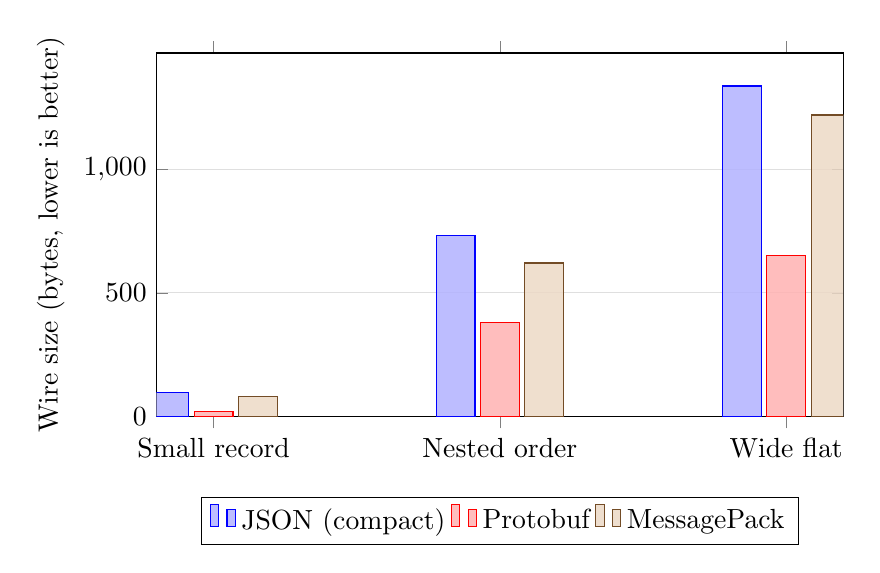
\begin{tikzpicture}
    \begin{axis}[
        ybar,
        width=0.85\textwidth,
        height=6.2cm,
        bar width=14pt,
        symbolic x coords={Small record, Nested order, Wide flat},
        xtick=data,
        ylabel={Wire size (bytes, lower is better)},
        ymin=0,
        legend style={at={(0.5,-0.22)}, anchor=north, legend columns=-1},
        ymajorgrids=true,
        grid style={gray!25},
        every axis plot/.append style={fill opacity=0.85}
      ]
      \addplot coordinates {(Small record, 98) (Nested order, 733) (Wide flat, 1336)};
      \addplot coordinates {(Small record, 20) (Nested order, 380) (Wide flat, 650)};
      \addplot coordinates {(Small record, 82) (Nested order, 621) (Wide flat, 1219)};
      \legend{JSON (compact), Protobuf, MessagePack}
    \end{axis}
  \end{tikzpicture}
  \caption{Wire sizes for three payload shapes. JSON and MessagePack bars are
           measured by the benchmark harness in Section~\ref{sec:ch4-code}; the
           protobuf small-record bar is measured (the hand-rolled codec), and the
           protobuf nested/wide bars are projected from packed-field arithmetic ---
           your lab run will refine them. Binary formats win consistently; the
           margin grows with numeric and wide payloads.}
  \label{fig:ch4-sizes}
\end{figure}

\begin{figure}[h]
  \centering
  \begin{tikzpicture}[
      font=\small,
      decision/.style={diamond, draw, aspect=2.2, align=center, inner sep=1pt, fill=blue!6},
      outcome/.style={rectangle, draw, rounded corners, align=center, fill=green!8, inner sep=4pt},
      every edge/.style={draw, -latex},
      node distance=0.9cm and 1.6cm]
    \node[decision] (browser) {Browser-facing or\\third-party public API?};
    \node[decision, below left=of browser] (stream) {Append-only streams /\\event log storage?};
    \node[decision, below right=of browser] (contract) {Strict cross-team\\contract + codegen?};
    \node[decision, below=of contract] (schemareg) {Schema registry\\available?};
    \node[outcome, left=of stream] (json) {\textbf{JSON}\\(+ JSON Schema)};
    \node[outcome, below=of stream] (avro) {\textbf{Avro}\\(writer schema + registry)};
    \node[outcome, right=of schemareg] (proto) {\textbf{Protobuf}\\(tags + reserved)};
    \node[outcome, below=of schemareg] (msgpack) {\textbf{MessagePack}\\(+ JSON Schema out-of-band)};
    \path (browser) edge node[above left]{yes} (json);
    \path (browser) edge node[above right]{no} (contract);
    \path (contract) edge node[left]{no, internal only} (stream);
    \path (stream) edge node[above]{yes} (avro);
    \path (stream) edge node[left]{no} (msgpack);
    \path (contract) edge node[right]{yes} (schemareg);
    \path (schemareg) edge node[above]{yes} (proto);
    \path (schemareg) edge node[left]{no} (msgpack);
  \end{tikzpicture}
  \caption{Format selection decision tree. Defaults, not laws: a public API with a
           performance-critical mobile tier may still serve protobuf via a vendor
           media type (Section~\ref{sec:ch4-negotiation}).}
  \label{fig:ch4-formattree}
\end{figure}

\subsection{Content Negotiation: Agreeing on the Bytes}
\label{sec:ch4-negotiation}

Serialization answers ``how do I encode this object?'' Content negotiation answers
the prior question: ``\emph{which} encoding, in which language, compressed how, does
this response carry?'' HTTP semantics (RFC~9110, Section~12) define proactive
negotiation via request headers the server evaluates against the representations it
can produce~\cite{rfc9110}.

\paragraph{\texttt{Accept} and q-values: the selection algorithm.}
The \texttt{Accept} header is a comma-separated list of \emph{media ranges} with
optional quality values:

\begin{minted}{text}
Accept: application/vnd.northwind.parts+json;v=2,
        application/json;q=0.9,
        text/html;q=0.8,
        application/*;q=0.5,
        */*;q=0.1
\end{minted}

A media range matches a concrete media type by specificity: an exact
\texttt{type/subtype} with parameters beats \texttt{type/*}, which beats
\texttt{*/*}. The server's algorithm --- which Section~\ref{sec:ch4-code} implements
--- is:

\begin{enumerate}
  \item Parse each entry into (type, subtype, parameters, $q$); a missing
        \texttt{q} means $q = 1.0$; a missing \texttt{Accept} header means
        \texttt{*/*} at $q = 1.0$.
  \item For each \emph{available representation}, find the most specific matching
        range; assign it that range's $q$. Entries with $q = 0$ mean ``explicitly
        refused''.
  \item Order candidates by descending $q$; break ties by media-range specificity
        (exact $>$ type-wildcard $>$ full wildcard), then by server preference.
  \item If nothing matches with $q > 0$, return \texttt{406 Not Acceptable}.
\end{enumerate}

Worked example: suppose the server can produce \texttt{application/json} and
\texttt{text/html} for the header above. \texttt{application/json} matches both the
\texttt{v=2} vendor range (no --- parameters don't match, the vendor subtype
differs), \texttt{application/json} at $q{=}0.9$, \texttt{application/*} at
$q{=}0.5$, and \texttt{*/*} at $q{=}0.1$; the most specific matching range is
\texttt{application/json} itself, so the score is $0.9$. \texttt{text/html} scores
$0.8$. The server selects JSON. Note what did \emph{not} happen: the vendor range
with its \texttt{v=2} parameter did not match plain \texttt{application/json} ---
parameter-bearing ranges match only representations that satisfy the parameters.

\paragraph{\texttt{Content-Type}, charset, and media type parameters.}
\texttt{Accept} is the request side; \texttt{Content-Type} is the response's
declaration of what the body \emph{actually is}:

\begin{minted}{text}
Content-Type: application/json; charset=utf-8
\end{minted}

Parameters after the semicolon are part of the type. \texttt{charset} governs how
bytes map to characters; omitting it from a text type invites the receiver to guess
(legacy defaults bite here --- e.g.\ ISO-8859-1 assumptions in old stacks). JSON in
UTF-8 needs no charset at all per RFC~8259~\cite{rfc8259}, but emitting
\texttt{charset=utf-8} explicitly is harmless and silences buggy intermediaries.

\paragraph{Vendor media types.}
Public APIs increasingly version \emph{representations} instead of URLs via vendor
trees:

\begin{minted}{text}
application/vnd.northwind.parts+json;v=2
\end{minted}

The \texttt{vnd.} tree marks a company-owned type; the \texttt{+json} suffix tells
generic tooling the body follows JSON structure (so a JSON Schema validator or a
pretty-printer works unmodified); the \texttt{v=2} parameter carries the contract
version. This keeps URLs stable (\texttt{GET /parts/NR-1001}) while the
representation evolves --- the purest expression of REST's
representation-orientation, and the pattern behind GitHub's and Stripe-style
content-negotiated versioning. The operational cost: caches must key on
\texttt{Accept} (via the \texttt{Vary} header), and intermediaries that ignore
parameters can serve a v1 body to a v2 client. Test your CDN.

\paragraph{\texttt{Accept-Encoding} and compression trade-offs.}
Independently of media type, the client advertises acceptable \emph{content
codings}:

\begin{minted}{text}
Accept-Encoding: br;q=1.0, gzip;q=0.8, zstd;q=0.9, identity;q=0.1
\end{minted}

\texttt{gzip} (DEFLATE) is universal; \texttt{br} (Brotli) compresses text 15--25\,\%
smaller at similar decode cost; \texttt{zstd} offers tunable levels with excellent
decode speed and is spreading through CDN and gRPC stacks. The engineering
trade-offs:

\begin{itemize}
  \item \textbf{CPU vs.\ bytes.} Compression pays when the link is the bottleneck
        (mobile, cross-region) and the payload is large and repetitive (JSON
        arrays). For sub-kilobyte payloads, compression \emph{adds} bytes (frame
        overhead) and CPU; most servers enforce a minimum size threshold
        (\textasciitilde860 bytes is a common nginx default; 1 KiB is a sane rule).
  \item \textbf{Compression bombs.} A 10~KB gzip body can expand to gigabytes of
        zeros. Any service that decompresses untrusted input must cap the
        \emph{decompressed} size mid-stream (Section~\ref{sec:ch4-pitfalls});
        Python's \texttt{gzip.decompress} has no built-in limit ---
        \texttt{gzip.GzipFile} with bounded \texttt{read(n)} loops does.
  \item \textbf{Streaming compression.} For large or unbounded bodies, compress
        chunk-by-chunk (\texttt{Content-Encoding: gzip} with chunked or HTTP/2
        framing) rather than buffering the whole payload; the client's memory stays
        flat and time-to-first-byte drops. Never combine with
        \texttt{Content-Length} --- the compressed length is unknown until done.
  \item \textbf{Double compression.} Binary formats and already-compressed media
        (images, \texttt{.parquet}, \texttt{.zip}) gain nothing; skip encoding for
        them to save CPU.
\end{itemize}

\begin{figure}[h]
  \centering
  \begin{tikzpicture}[
      font=\small,
      startstop/.style={rectangle, rounded corners, draw, align=center, fill=blue!7, inner sep=4pt},
      decision/.style={diamond, draw, aspect=2.4, align=center, fill=yellow!10, inner sep=1pt},
      outcome/.style={rectangle, draw, align=center, fill=green!8, inner sep=4pt},
      every edge/.style={draw, -latex},
      node distance=0.75cm and 1.1cm]
    \node[startstop] (req) {Request arrives\\\texttt{Accept} + \texttt{Accept-Encoding}};
    \node[decision, below=of req] (parse) {Parse ranges;\\any $q>0$ match\\for a producible type?};
    \node[outcome, right=1.6cm of parse] (err) {\texttt{406 Not Acceptable}\\(+\texttt{Accept-Post} hints)};
    \node[startstop, below=of parse] (best) {Select best match:\\max $q$, then specificity,\\then server preference};
    \node[decision, below=of best] (enc) {Shared coding with\\$q>0$ and body\\over threshold?};
    \node[outcome, right=1.6cm of enc] (plain) {Send identity body\\\texttt{Content-Type} + \texttt{Vary: Accept}};
    \node[startstop, below=of enc] (compress) {Stream-compress (gzip/br/zstd)\\\texttt{Content-Encoding} + \texttt{Vary: Accept, Accept-Encoding}};
    \node[startstop, below=of compress] (done) {Log negotiated type + coding\\(observability: negotiation miss rate)};
    \path (req) edge (parse);
    \path (parse) edge node[above]{no} (err);
    \path (parse) edge node[right]{yes} (best);
    \path (best) edge (enc);
    \path (enc) edge node[above]{no} (plain);
    \path (enc) edge node[right]{yes} (compress);
    \path (compress) edge (done);
    \path (plain) |- (done.east);
  \end{tikzpicture}
  \caption{Server-side negotiation decision flow. The \texttt{Vary} header is what
           keeps shared caches honest across negotiated variants.}
  \label{fig:ch4-negflow}
\end{figure}

\begin{figure}[h]
  \centering
  \begin{tikzpicture}[
      font=\small,
      stage/.style={rectangle, draw, rounded corners, align=center, fill=blue!6, inner sep=5pt, minimum width=2.5cm},
      data/.style={rectangle, draw, dashed, align=center, fill=gray!8, inner sep=4pt},
      every edge/.style={draw, -latex},
      node distance=0.55cm]
    \node[data] (obj) {In-memory object\\(Part dataclass)};
    \node[stage, right=of obj] (validate) {Validate against\\contract (schema)};
    \node[stage, right=of validate] (encode) {Encode\\(JSON / proto / Avro)};
    \node[stage, right=of encode] (compress) {Optional\\compression};
    \node[data, right=of compress] (wire) {Wire bytes\\(+ \texttt{Content-Type})};
    \node[stage, below=0.7cm of compress] (decompress) {Bounded\\decompression};
    \node[stage, left=of decompress] (decode) {Decode\\(reader schema / tags)};
    \node[stage, left=of decode] (revalidate) {Re-validate at\\trust boundary};
    \node[data, left=of revalidate] (obj2) {Reconstructed\\object};
    \path (obj) edge (validate);
    \path (validate) edge (encode);
    \path (encode) edge (compress);
    \path (compress) edge (wire);
    \path (wire.south) |- (decompress.east);
    \path (decompress) edge (decode);
    \path (decode) edge (revalidate);
    \path (revalidate) edge (obj2);
  \end{tikzpicture}
  \caption{Encode/decode pipeline. Symmetric validation at both trust boundaries is
           deliberate: the producer's bug must not become the consumer's incident.}
  \label{fig:ch4-pipeline}
\end{figure}

\subsection{Contract Engineering: Registries, Compatibility, Consumers}
\label{sec:ch4-compat}

A schema only creates value if every producer and consumer agrees on \emph{which}
schema and on \emph{how it may change}. That agreement system has three pillars.

\paragraph{Schema registries.}
A registry (Confluent Schema Registry for Avro/Protobuf/JSON Schema, or an internal
artifact store keyed by \texttt{\$id}) is a versioned, addressable store of schemas
plus a \emph{compatibility gate}: every new schema version is checked against the
configured compatibility mode before it may be published. Producers reference
schemas by ID (Avro's wire convention prefixes each message with a 4-byte registry
ID), so payloads stay lean and consumers fetch-and-cache schemas out of band.

\begin{definition}[Compatibility modes]
Given existing consumers $C$ and producers $P$ of a schema $S$, and a candidate new
schema $S'$:
\begin{itemize}
  \item \textbf{Backward compatible:} consumers written for $S'$ can read data
        written with $S$ (the \emph{new code reads old data}). Typical allowed
        change: add a field \emph{with a default}, delete a field. Required for
        consumers to upgrade first.
  \item \textbf{Forward compatible:} consumers written for $S$ can read data written
        with $S'$ (the \emph{old code reads new data}). Typical allowed change:
        delete a field with a default, add a field that old readers ignore. Required
        for producers to upgrade first.
  \item \textbf{Full compatible:} both directions simultaneously --- changes are
        restricted to optional-field additions/removals with defaults. The only mode
        that permits arbitrary upgrade order in a fleet.
\end{itemize}
\end{definition}

The modes compose transitively across versions (\emph{backward-transitive} checks
$S'$ against \emph{all} earlier versions, not just the latest) --- essential when
old data lives for years in a log or a data lake.

\paragraph{Consumer-driven contracts.}
Compatibility modes answer ``is this schema change structurally safe?'' They cannot
answer ``will I break the mobile app's checkout screen?'' --- that requires knowing
what consumers actually \emph{use}. \textbf{Consumer-driven contract testing} (CDC)
records each consumer's expectations as executable contracts and runs them against
provider builds in CI, flipping the power balance: providers discover breaking
changes before merge, and consumers own the definition of ``breaking''. We treat
CDC in full --- Pact-style workflows, contract storage, provider verification --- in
Chapter~19 (Testing \& Quality Engineering). For now, hold the principle: the
contract is co-owned, executable, and versioned alongside the code.

\begin{examplebox}
\textbf{Contract-first change workflow at Northwind Robotics (parts service).}
(1)~Schema author proposes \texttt{part-v3.json} adding optional
\texttt{firmware\_channel}. (2)~CI validates the schema itself, then runs the
registry check: backward-compatible? yes (optional field, default
\texttt{"stable"}). (3)~Provider CI runs recorded consumer contracts --- one
consumer's contract forbids unknown top-level keys, so the change is negotiated to
arrive under \texttt{additionalProperties}-tolerant semantics first.
(4)~Schema published; producer and consumer deploy in either order. No runtime
surprises, because every gate was executable.
\end{examplebox}

%% ----------------------------------------------------------------------------
\section{Production-Ready Code Implementation}
\label{sec:ch4-code}

Five complete, typed, offline programs. All run under Python 3.11+; only the JSON
Schema pipeline and (optionally) the benchmark need third-party packages
(Section~\ref{sec:ch4-deps}). All fixtures are synthetic Northwind Robotics data;
all demos use deterministic seeds.

\subsection{A Hand-Rolled Protobuf Codec (Pure Standard Library)}
\label{sec:ch4-code-proto}

The pedagogical centerpiece: a working encoder/decoder for the \texttt{Part}
message from Section~\ref{sec:ch4-protobuf}, using nothing but \texttt{struct} and
\texttt{dataclasses}. Reading this code \emph{is} reading the wire format
specification~\cite{protobufdocs}.

\begin{minted}{python}
"""mini_protobuf.py -- a hand-rolled Protocol Buffers wire-format codec.

Implements (proto3 semantics) for a single message:
    message Part {
      string part_id  = 1;  // LEN     wire type 2
      uint32 qty      = 2;  // VARINT  wire type 0
      sint32 delta    = 3;  // VARINT  wire type 0 (zigzag)
      double unit_kg  = 4;  // I64     wire type 1
      float  width_mm = 5;  // I32     wire type 5
    }
Pure standard library; offline; deterministic. Python 3.11+.
"""
from __future__ import annotations

import struct
from dataclasses import dataclass

WIRE_VARINT = 0
WIRE_I64 = 1
WIRE_LEN = 2
WIRE_I32 = 5
_MAX_VARINT_BYTES = 10  # a 64-bit varint never exceeds 10 bytes


class DecodeError(ValueError):
    """Raised when a byte stream is not a valid Part encoding."""


def encode_varint(value: int) -> bytes:
    """Encode an unsigned 64-bit integer as a varint (7 bits/byte, LSB first)."""
    if not 0 <= value < 1 << 64:
        raise ValueError(f"varint out of uint64 range: {value}")
    out = bytearray()
    while True:
        bits = value & 0x7F
        value >>= 7
        out.append(bits | 0x80 if value else bits)  # MSB set => more bytes
        if not value:
            return bytes(out)


def decode_varint(buf: bytes, pos: int) -> tuple[int, int]:
    """Decode a varint at buf[pos:]; return (value, next_pos)."""
    result, shift = 0, 0
    for i in range(_MAX_VARINT_BYTES):
        if pos + i >= len(buf):
            raise DecodeError("truncated varint")
        byte = buf[pos + i]
        result |= (byte & 0x7F) << shift
        if not byte & 0x80:  # continuation bit clear => final byte
            return result, pos + i + 1
        shift += 7
    raise DecodeError("varint exceeds 64 bits")


def zigzag_encode(n: int) -> int:
    """Map signed n to unsigned so small magnitudes stay short."""
    return (n << 1) ^ (n >> 63)


def zigzag_decode(u: int) -> int:
    return (u >> 1) ^ -(u & 1)


def make_tag(field_number: int, wire_type: int) -> bytes:
    if not 1 <= field_number < 1 << 29:
        raise ValueError(f"field number out of range: {field_number}")
    return encode_varint((field_number << 3) | wire_type)


@dataclass(frozen=True)
class Part:
    part_id: str = ""
    qty: int = 0
    delta: int = 0
    unit_kg: float = 0.0
    width_mm: float = 0.0

    def encode(self) -> bytes:
        """Serialize; proto3 rule: default-valued scalar fields are omitted."""
        out = bytearray()
        if self.part_id:
            raw = self.part_id.encode("utf-8")
            out += make_tag(1, WIRE_LEN) + encode_varint(len(raw)) + raw
        if self.qty:
            out += make_tag(2, WIRE_VARINT) + encode_varint(self.qty)
        if self.delta:
            out += make_tag(3, WIRE_VARINT) + encode_varint(zigzag_encode(self.delta))
        if self.unit_kg != 0.0:
            out += make_tag(4, WIRE_I64) + struct.pack("<d", self.unit_kg)
        if self.width_mm != 0.0:
            out += make_tag(5, WIRE_I32) + struct.pack("<f", self.width_mm)
        return bytes(out)

    @classmethod
    def decode(cls, buf: bytes) -> "Part":
        """Parse wire bytes. Unknown fields are skipped (forward compat)."""
        part_id, qty, delta, unit_kg, width_mm = "", 0, 0, 0.0, 0.0
        pos = 0
        while pos < len(buf):
            tag, pos = decode_varint(buf, pos)
            field_number, wire_type = tag >> 3, tag & 0b111
            if wire_type == WIRE_VARINT:
                value, pos = decode_varint(buf, pos)
                if field_number == 2:
                    qty = value
                elif field_number == 3:
                    delta = zigzag_decode(value)
            elif wire_type == WIRE_LEN:
                length, pos = decode_varint(buf, pos)
                if pos + length > len(buf):
                    raise DecodeError("LEN field overruns buffer")
                payload = buf[pos:pos + length]
                pos += length
                if field_number == 1:
                    part_id = payload.decode("utf-8")
            elif wire_type == WIRE_I64:
                (value,) = struct.unpack_from("<d", buf, pos)
                pos += 8
                if field_number == 4:
                    unit_kg = value
            elif wire_type == WIRE_I32:
                (value,) = struct.unpack_from("<f", buf, pos)
                pos += 4
                if field_number == 5:
                    width_mm = value
            else:
                raise DecodeError(f"unsupported wire type {wire_type}")
        return cls(part_id=part_id, qty=qty, delta=delta,
                   unit_kg=unit_kg, width_mm=width_mm)


def _demo() -> None:
    part = Part(part_id="A1", qty=300, delta=-3, unit_kg=1.5, width_mm=42.0)
    wire = part.encode()
    print(f"Encoded {len(wire)} bytes:")
    for i, byte in enumerate(wire):
        print(f"  offset {i:2d}: 0x{byte:02X}  0b{byte:08b}")
    roundtrip = Part.decode(wire)
    assert roundtrip == part, "round-trip mismatch"
    # The varint for qty=300 must be exactly the textbook pair 0xAC 0x02:
    assert wire[5:7] == bytes([0xAC, 0x02])
    # zigzag(-3) == 5 must occupy a single byte after the field-3 tag:
    assert wire[7] == 0x18 and wire[8] == 0x05
    # Unknown-field tolerance: append field 99 (VARINT) and re-decode.
    tolerant = Part.decode(wire + make_tag(99, WIRE_VARINT) + encode_varint(7))
    assert tolerant == part
    print("Round-trip OK; varint, zigzag, and unknown-field checks passed.")


if __name__ == "__main__":
    _demo()
\end{minted}

Expected output (abridged): the encoder emits 23 bytes; offset 5--6 print
\texttt{0xAC}, \texttt{0x02} (the worked varint for 300); offset 8 prints
\texttt{0x05} (zigzag of $-3$); all assertions pass.

\subsection{JSON Schema Validation Pipeline with RFC 9457 Errors}
\label{sec:ch4-code-schema}

Validating is easy; producing \emph{actionable, standard-shaped} errors is the
production part. This pipeline validates Northwind \texttt{Part} payloads against a
2020-12 schema and renders failures as an RFC~9457
\texttt{application/problem+json} document~\cite{rfc9457, jsonschemadocs}.

\begin{minted}{python}
"""validate_parts.py -- JSON Schema 2020-12 validation -> RFC 9457 errors.

Requires: jsonschema>=4.21 (see Python Dependencies Appendix).
Offline: the schema is an embedded fixture; no registry, no network.
"""
from __future__ import annotations

import json
import logging
from typing import Any

from jsonschema import Draft202012Validator
from jsonschema.exceptions import SchemaError

logger = logging.getLogger("northwind.validation")

PART_SCHEMA: dict[str, Any] = {
    "$schema": "https://json-schema.org/draft/2020-12/schema",
    "$id": "https://schemas.northwind-robotics.example/parts/v2/part.json",
    "title": "Northwind Robotics Part",
    "type": "object",
    "properties": {
        "part_id": {
            "type": "string",
            "pattern": "^NR-[0-9]{4}$",
            "description": "Catalog identifier; string to avoid the 2^53 trap.",
        },
        "name": {"type": "string", "minLength": 1, "maxLength": 120},
        "qty": {"type": "integer", "minimum": 0},
        "unit_price_usd": {"type": "number", "exclusiveMinimum": 0},
        "status": {"enum": ["active", "deprecated", "eol"]},
        "firmware": {"type": "string"},
    },
    "required": ["part_id", "name", "qty", "status"],
    "additionalProperties": False,
}


def build_validator(schema: dict[str, Any]) -> Draft202012Validator:
    """Compile the schema once; fail fast if the schema itself is invalid."""
    try:
        Draft202012Validator.check_schema(schema)
    except SchemaError as exc:
        raise ValueError(f"schema is not valid 2020-12: {exc.message}") from exc
    return Draft202012Validator(schema)


def to_problem_details(
    validator: Draft202012Validator, instance: Any
) -> dict[str, Any] | None:
    """Return None if valid, else an RFC 9457 problem document (status 422)."""
    errors = sorted(validator.iter_errors(instance), key=lambda e: list(e.path))
    if not errors:
        return None
    return {
        "type": "https://problems.northwind-robotics.example/schema-validation",
        "title": "Payload does not conform to the Part schema",
        "status": 422,
        "detail": f"{len(errors)} schema violation(s) found.",
        "instance": "/v2/parts",
        "errors": [
            {
                "pointer": "/" + "/".join(str(p) for p in e.absolute_path),
                "keyword": e.validator,
                "message": e.message,
            }
            for e in errors
        ],
    }


def _demo() -> None:
    logging.basicConfig(level=logging.INFO, format="%(levelname)s %(message)s")
    validator = build_validator(PART_SCHEMA)

    good = {
        "part_id": "NR-1001", "name": "Servo Motor 42mm",
        "qty": 120, "unit_price_usd": 18.75, "status": "active",
    }
    bad = {
        "part_id": "servo-1",          # violates pattern
        "name": "",                    # violates minLength
        "qty": -4,                     # violates minimum
        "status": "retired",           # not in enum
        "debug_note": "leftover",      # additionalProperties: false
    }
    assert to_problem_details(validator, good) is None
    problem = to_problem_details(validator, bad)
    assert problem is not None and problem["status"] == 422
    body = json.dumps(problem, indent=2)
    logger.info("responding 422 with application/problem+json")
    print(body)
    assert len(problem["errors"]) == 5  # one per violation, all collected


if __name__ == "__main__":
    _demo()
\end{minted}

Note the deliberate choices: the validator is compiled once (schema compilation is
expensive; per-request compilation is an anti-pattern), \texttt{iter\_errors}
collects \emph{all} violations, and each violation carries a JSON Pointer
(\texttt{pointer}) so clients can highlight the offending field.

\subsection{A Content-Negotiation Selector (Pure Standard Library)}
\label{sec:ch4-code-negotiation}

The \texttt{Accept} algorithm from Section~\ref{sec:ch4-negotiation}, implemented
exactly, with unit-test-style asserts covering q-values, specificity, and
\texttt{q=0} refusal~\cite{rfc9110}.

\begin{minted}{python}
"""negotiation.py -- RFC 9110 proactive content negotiation, pure stdlib."""
from __future__ import annotations

from dataclasses import dataclass


@dataclass(frozen=True)
class MediaRange:
    type: str
    subtype: str
    q: float = 1.0

    def specificity(self) -> int:
        """exact(2) > type/* (1) > */* (0); drives tie-breaking."""
        if self.type == "*":
            return 0
        if self.subtype == "*":
            return 1
        return 2

    def matches(self, media_type: str) -> bool:
        t, _, s = media_type.partition("/")
        return (self.type in ("*", t)) and (self.subtype in ("*", s))


def parse_accept(header: str | None) -> list[MediaRange]:
    """Parse an Accept header; absent or blank means '*/*' at q=1.0."""
    if not header or not header.strip():
        return [MediaRange("*", "*")]
    ranges: list[MediaRange] = []
    for raw in header.split(","):
        parts = [p.strip() for p in raw.split(";")]
        type_, _, subtype = parts[0].partition("/")
        if not subtype:
            continue  # malformed entry: skip, do not crash on client junk
        q = 1.0
        for param in parts[1:]:
            key, _, value = param.partition("=")
            if key.strip().lower() == "q":
                try:
                    q = float(value)
                except ValueError:
                    q = 0.0  # a non-numeric q is treated as 'refuse'
        q = min(max(q, 0.0), 1.0)
        ranges.append(MediaRange(type_.strip().lower(),
                                 subtype.strip().lower(), q))
    return ranges or [MediaRange("*", "*")]


def select_representation(
    accept_header: str | None, available: list[str]
) -> str | None:
    """Return the best available media type, or None (-> HTTP 406).

    Score = q of the MOST SPECIFIC matching range; ties break toward
    the server's own preference (the order of `available`).
    """
    if not available:
        raise ValueError("available must contain at least one media type")
    ranges = parse_accept(accept_header)
    scored: list[tuple[float, int, int, str]] = []
    for server_rank, media_type in enumerate(available):
        matches = [r for r in ranges if r.matches(media_type)]
        if not matches:
            scored.append((0.0, 0, -server_rank, media_type))
            continue
        best = max(matches, key=lambda r: (r.specificity(), r.q))
        scored.append((best.q, best.specificity(), -server_rank, media_type))
    scored.sort(reverse=True)
    top_q, _, _, winner = scored[0]
    return winner if top_q > 0.0 else None


def _demo() -> None:
    header = ("application/vnd.northwind.parts+json;v=2, "
              "application/json;q=0.9, text/html;q=0.8, */*;q=0.1")
    server = ["application/json", "text/html"]
    assert select_representation(header, server) == "application/json"
    assert select_representation("text/html", server) == "text/html"
    # q=0 on everything the server can do -> 406 (None)
    assert select_representation("image/png, application/json;q=0",
                                 server) is None
    # No Accept header -> server default (first listed)
    assert select_representation(None, server) == "application/json"
    # Specificity trap: JSON is scored by the MORE SPECIFIC application/*
    # range (q=0.4), not by the */* range (q=0.9) -> HTML wins at 0.9.
    assert select_representation("application/*;q=0.4, */*;q=0.9",
                                 server) == "text/html"
    print("All negotiation selector checks passed.")


if __name__ == "__main__":
    _demo()
\end{minted}

\begin{warningbox}
The final assert encodes the subtlest rule in RFC~9110 negotiation: a
representation's quality is taken from the \emph{most specific} media range that
matches it --- not the highest-q range. Given \texttt{application/*;q=0.4,
*/*;q=0.9}, JSON is scored $0.4$ (the type-wildcard range) even though the full
wildcard offers $0.9$; HTML, matched only by \texttt{*/*}, keeps $0.9$ and wins.
A ``max q anywhere'' implementation silently inverts client intent here. This is
exactly the kind of edge case your own selector must be unit-tested against.
\end{warningbox}

\subsection{A Deterministic Serialization Benchmark Harness}
\label{sec:ch4-code-bench}

Benchmarks are where format debates go to be settled honestly. The harness below
builds three deterministic payload shapes (small record, nested order, wide flat),
round-trips each through JSON, the hand-rolled protobuf codec, and --- if installed
--- MessagePack, and prints a size + timing table. Structure is fully deterministic
(seeded \texttt{random}); timings are reported, never asserted.

\begin{minted}{python}
"""bench_serializers.py -- JSON vs hand-rolled Protobuf vs MessagePack.

Deterministic fixtures (seeded), fixed iteration counts, illustrative timing.
MessagePack is optional: if msgpack is not installed, its column is skipped.
Run:  python bench_serializers.py
"""
from __future__ import annotations

import json
import random
import time
from dataclasses import dataclass
from typing import Any, Callable

from mini_protobuf import Part  # the hand-rolled codec from Listing 1

try:
    import msgpack  # type: ignore[import-not-found]
except ImportError:  # pragma: no cover - optional dependency
    msgpack = None  # type: ignore[assignment]

ITERATIONS = 5_000


def build_fixtures(seed: int = 42) -> dict[str, dict[str, Any]]:
    rng = random.Random(seed)
    small = {"part_id": "NR-1001", "name": "Servo Motor 42mm",
             "qty": 120, "unit_price_usd": 18.75, "status": "active"}
    nested = {
        "order_id": "9007199254740991",  # string on purpose: see 2^53 rule
        "customer": {"id": "C-88213", "region": "MX-NLE"},
        "lines": [{"part_id": f"NR-{1000 + i}", "qty": rng.randint(1, 50),
                   "unit_price_usd": round(rng.uniform(1, 200), 2)}
                  for i in range(12)],
    }
    wide = {f"metric_{i:02d}": round(rng.uniform(0, 1000), 4) for i in range(64)}
    return {"small_record": small, "nested_order": nested, "wide_flat": wide}


@dataclass(frozen=True)
class Codec:
    name: str
    encode: Callable[[dict[str, Any]], bytes]
    decode: Callable[[bytes], Any]


def _json_codecs() -> Codec:
    return Codec("json",
                 lambda d: json.dumps(d, separators=(",", ":")).encode("utf-8"),
                 lambda b: json.loads(b.decode("utf-8")))


def _msgpack_codecs() -> Codec | None:
    if msgpack is None:
        return None
    return Codec("msgpack",
                 lambda d: msgpack.packb(d, use_bin_type=True),
                 lambda b: msgpack.unpackb(b, raw=False))


def _proto_small_codec() -> Codec:
    """Protobuf comparison for the small-record shape (Part fields only)."""
    def enc(d: dict[str, Any]) -> bytes:
        return Part(part_id=d["part_id"], qty=d["qty"],
                    unit_kg=d["unit_price_usd"]).encode()

    def dec(b: bytes) -> Part:
        return Part.decode(b)
    return Codec("mini-protobuf", enc, dec)


def timed(fn: Callable[[], Any], iterations: int = ITERATIONS) -> float:
    """Median-ish wall time per call in microseconds (illustrative only)."""
    start = time.perf_counter()
    for _ in range(iterations):
        fn()
    return (time.perf_counter() - start) * 1e6 / iterations


def main() -> None:
    fixtures = build_fixtures()
    generic = [c for c in (_json_codecs(), _msgpack_codecs()) if c]
    header = f"{'shape':<14}{'codec':<15}{'bytes':>8}{'enc us':>10}{'dec us':>10}"
    print(header)
    print("-" * len(header))
    for shape, doc in fixtures.items():
        codecs = list(generic)
        if shape == "small_record":
            codecs.append(_proto_small_codec())
        for codec in codecs:
            wire = codec.encode(doc)
            assert codec.decode(wire) is not None
            enc_us = timed(lambda: codec.encode(doc))
            dec_us = timed(lambda: codec.decode(wire))
            print(f"{shape:<14}{codec.name:<15}{len(wire):>8}"
                  f"{enc_us:>10.2f}{dec_us:>10.2f}")


if __name__ == "__main__":
    main()
\end{minted}

The protobuf row covers only the small-record shape because our hand-rolled codec
models exactly one message --- extending it is Capstone~3. Sizes in
Figure~\ref{fig:ch4-sizes} come from this harness; expect the same ordering and
different absolute numbers on your machine.

\subsection{Streaming NDJSON Writer/Reader}
\label{sec:ch4-code-ndjson}

A line-delimited pipeline with bounded memory: the writer emits one JSON value per
line; the reader is a generator, so the consumer controls the pace ---
backpressure-friendly by construction. A malformed line is logged and skipped, not
fatal: stream consumers must survive one poisoned record.

\begin{minted}{python}
"""ndjson_stream.py -- streaming JSON Lines writer/reader (stdlib only)."""
from __future__ import annotations

import io
import json
import logging
from typing import Any, Iterator, TextIO

logger = logging.getLogger("northwind.ndjson")


def write_ndjson(records: Iterator[dict[str, Any]], sink: TextIO) -> int:
    """Write records as NDJSON; returns the number of lines written."""
    count = 0
    for record in records:
        line = json.dumps(record, separators=(",", ":"), ensure_ascii=False)
        if "\n" in line:  # json.dumps never emits raw newlines; guard anyway
            raise ValueError("record would break line framing")
        sink.write(line + "\n")
        count += 1
    sink.flush()
    return count


def read_ndjson(source: TextIO, max_line_bytes: int = 1_000_000) -> Iterator[Any]:
    """Yield one decoded value per line. Bounded lines; bad lines are skipped.

    Backpressure: this is a generator -- if the consumer is slow, no records
    are pulled from `source`, so memory stays O(1) in the number of records.
    """
    for lineno, raw in enumerate(source, start=1):
        if len(raw) > max_line_bytes:
            logger.error("line %d exceeds %d bytes; skipping",
                         lineno, max_line_bytes)
            continue
        line = raw.strip()
        if not line:
            continue
        try:
            yield json.loads(line)
        except json.JSONDecodeError as exc:
            logger.error("line %d is not valid JSON (%s); skipping",
                         lineno, exc.msg)


def _demo() -> None:
    logging.basicConfig(level=logging.INFO, format="%(levelname)s %(message)s")
    records = (
        {"part_id": f"NR-{1000 + i}", "qty": i * 7, "status": "active"}
        for i in range(1, 4)
    )
    buffer = io.StringIO()  # stands in for a socket or a log file
    written = write_ndjson(records, buffer)
    # Simulate one poisoned record appended after the clean batch:
    buffer.write('{"part_id": "BROKEN", "qty": ')
    buffer.seek(0)
    decoded = list(read_ndjson(buffer))
    assert written == 3
    assert [r["part_id"] for r in decoded] == ["NR-1001", "NR-1002", "NR-1003"]
    assert sum(r["qty"] for r in decoded) == 7 + 14 + 21
    print(f"Wrote {written} lines; recovered {len(decoded)} of "
          f"{written + 1} (1 poisoned line skipped).")


if __name__ == "__main__":
    _demo()
\end{minted}

\begin{keyconceptbox}
Backpressure in a pull-based pipeline is free: because \texttt{read\_ndjson} is a
generator, records flow only as fast as the consumer iterates. The expensive
resources --- the file handle, the socket buffer --- are held open but never
inflated. The dual discipline is on the writer: flush deliberately, and never emit
a record you have not finished framing (a torn write mid-line is the classic NDJSON
corruption when a process is killed; write-then-fsync per batch, or use atomic
file rotation as in Capstone~1).
\end{keyconceptbox}

%% ----------------------------------------------------------------------------
\section{Common Pitfalls \& Anti-Patterns}
\label{sec:ch4-pitfalls}

Each entry below is a defect class observed repeatedly in production systems, with
its mechanism and its fix.

\paragraph{1. Floats for money.}
\texttt{unit\_price\_usd: 19.99} is a binary approximation:
$19.99$ has no finite binary expansion, and \texttt{json.loads("19.99") ==
19.99} is true only because Python's repr round-trips; arithmetic
(\texttt{0.1 + 0.2 != 0.3}) does not. \textbf{Fix:} transmit money as integer minor
units (\texttt{unit\_price\_cents: 1999}) or as a decimal string parsed into
\texttt{decimal.Decimal}; in protobuf use a \texttt{Money}-style message, never
\texttt{float}/\texttt{double}.

\paragraph{2. Trusting \texttt{Content-Type} without sniffing the body.}
The header is a claim, not a fact. A compromised or buggy upstream can label
executable HTML as \texttt{application/json} and hand your parser --- or your
user's browser --- a different document than promised. \textbf{Fix:} validate the
body against the declared type (parse strictly, schema-validate at trust
boundaries), and send \texttt{X-Content-Type-Options: nosniff} on responses so
browsers do not second-guess you.

\paragraph{3. Reusing a protobuf tag number.}
The decoder resolves meaning solely by tag; a recycled tag makes old data silently
parse as a new field (Section~\ref{sec:ch4-lab} case study). \textbf{Fix:}
\texttt{reserved} statements, lint rules in CI, and a schema registry that diffs
tag allocations.

\paragraph{4. Unbounded decompression.}
\texttt{gzip.decompress(body)} on attacker-controlled input is a memory-exhaustion
primitive: a 42~KB bomb expands to 4.5~PB in the famous \texttt{42.zip}; even
honest 10~GB log archives arrive mislabeled. \textbf{Fix:} stream through
\texttt{gzip.GzipFile}/\texttt{zstandard} readers and abort when the cumulative
decompressed size crosses a configured ceiling; reject
\texttt{Content-Encoding} you did not negotiate.

\paragraph{5. Assuming JSON object key order.}
RFC~8259 defines objects as \emph{unordered}~\cite{rfc8259}. Python's
\texttt{dict} preserves insertion order, which makes order-dependent tests pass in
Python and fail against a Go intermediary that re-serializes with sorted keys, or a
CDN that normalizes payloads. \textbf{Fix:} never key logic on member order; if a
signature must cover the body, canonicalize (e.g.\ JCS, RFC~8785) before hashing.

\paragraph{6. Silent numeric coercion of identifiers.}
Serializing a database \texttt{BIGINT} primary key as a JSON number invites the
$2^{53}$ corruption from Section~\ref{sec:ch4-json}. ORM defaults do this to you
without asking. \textbf{Fix:} identifiers are strings by policy; schemas pin
\texttt{"type": "string"} with a pattern; linters reject \texttt{integer} schema
types on \texttt{*\_id} fields unless \texttt{maximum} $\le 2^{53}-1$ is declared.

\paragraph{7. \texttt{default} as a data-filling mechanism.}
JSON Schema's \texttt{default} is an \emph{annotation}; validators do not mutate
instances (Section~\ref{sec:ch4-jsonschema}). Pipelines that assume defaults were
applied read \texttt{None} downstream. \textbf{Fix:} apply defaults in application
code or with an explicit coercion pass; never rely on the validator to fix data.

\paragraph{8. Catching everything around the parser.}
\texttt{except Exception: return \{\}} converts a malformed-payload bug into a
phantom empty document, corrupting state silently. \textbf{Fix:} catch
\texttt{json.JSONDecodeError} (or your codec's specific error), map to a 400/422
problem document~\cite{rfc9457}, and let truly unexpected exceptions surface.

%% ----------------------------------------------------------------------------
\section{Hands-On Production Lab \& Real-World Case Study}
\label{sec:ch4-lab}

\subsection{Lab: Benchmark Three Formats and Produce a Decision Table}

\textbf{Objective.} Replace opinion with measurement: quantify JSON vs.\ protobuf
vs.\ MessagePack on \emph{your} payload shapes and turn the result into a selection
table your team could actually adopt.

\textbf{Setup (PowerShell).}
\begin{minted}{bash}
cd "C:\Training\Training Areas\Data jobs learning\APIs - Usage and development\code"
python -m venv .venv
.\.venv\Scripts\Activate.ps1
pip install -r requirements.txt   # jsonschema, msgpack (orjson optional)
python bench_serializers.py
\end{minted}

\textbf{Steps.}
\begin{enumerate}
  \item Run the harness from Listing in Section~\ref{sec:ch4-code-bench} unmodified;
        record the size column for all three shapes.
  \item Extend the fixtures: add a \texttt{deep\_tree} shape (6 levels of nesting)
        and a \texttt{text\_heavy} shape (8 KB of log message strings). Re-run.
  \item Extend the protobuf comparison: write a second hand-rolled codec for the
        \texttt{wide\_flat} shape as a \texttt{repeated double} packed field (wire
        type 2, one tag, then a length, then contiguous 8-byte values). Observe
        what packed encoding does to size and decode time.
  \item Add gzip on top of each format (\texttt{gzip.compress(wire, 9)}) and record
        the compressed sizes. Note which format compresses \emph{least} proportionally
        and explain why from the byte layouts you now understand.
  \item Produce a decision table with one row per shape and columns: raw size per
        format, gzip size per format, encode/decode time rank, debuggability note,
        and your recommended format for that shape \emph{in a named Northwind
        service} (e.g.\ public catalog API vs.\ internal telemetry bus).
\end{enumerate}

\textbf{Acceptance criteria.} Your table covers $\ge 5$ shapes $\times$ 3 formats;
every claim in the ``recommended'' column cites a number from your own run; the
report includes one paragraph explaining a result that surprised you.

\subsection{Case Study: The $2^{53}$ Order-ID Corruption Incident}

Northwind Robotics' orders service stores \texttt{order\_id} as a 64-bit integer
(a \texttt{BIGINT} identity column). The Java backend serializes it as a JSON
number --- correctly, per its own parser, which handles 64-bit integers natively.
Years pass. Then order volumes cross $2^{53}$, and the React storefront begins
silently routing customers to the wrong order-status pages: JavaScript's
\texttt{JSON.parse} reads every ID through an IEEE~754 double, and
\texttt{9007199254740993} and \texttt{9007199254740992} collapse to the same value
(Section~\ref{sec:ch4-json}). No errors, no alerts; the corruption is discovered
by a customer who reports seeing a stranger's shipment.

The postmortem's lessons, in the team's own remediation order: (1)~identifiers are
\emph{opaque strings} --- the API contract changed to
\texttt{"order\_id": "9007199254740993"}, shipped behind a vendor media type bump
\texttt{application/vnd.northwind.orders+json;v=2} with the negotiation machinery
of Section~\ref{sec:ch4-negotiation} serving both versions during the migration
window; (2)~the JSON Schema now declares every \texttt{*\_id} as a string with a
pattern, enforced in CI by the pipeline from Section~\ref{sec:ch4-code-schema};
(3)~a synthetic \emph{canary assertion} in staging posts IDs near $2^{53} \pm k$
and diffs what the browser receives; (4)~the team adopted a policy that numeric
JSON fields carry explicit \texttt{minimum}/\texttt{maximum} bounds, making the
safe range part of the reviewed contract rather than an implicit hope.

\begin{warningbox}
The incident's root cause was not ``JavaScript is bad at integers.'' It was a
contract that encoded a 64-bit semantic type into a format whose common
denominator cannot carry it, with no schema and no negotiation to catch the
mismatch. Serialization choices are contract choices.
\end{warningbox}

%% ----------------------------------------------------------------------------
\section{Self-Assessment Exercises \& Deep-Dive Questions}
\label{sec:ch4-exercises}

\begin{enumerate}[label=\textbf{E4.\arabic*}, leftmargin=1.5cm]
  \item Write out, by hand, the varint encoding of 1, 127, 128, and 16{,}384.
        Verify each with \texttt{encode\_varint} from the hand-rolled codec.
  \item Compute $\text{zigzag}(-64)$ and $\text{zigzag}^{-1}(127)$ without a
        computer; then check with \texttt{zigzag\_encode}/\texttt{zigzag\_decode}.
  \item A colleague proposes changing field 4 of \texttt{Part} from
        \texttt{double} (I64) to \texttt{int64} (VARINT) ``to save bytes.'' Using
        only the wire-type table, explain what old consumers will do with new data
        and why this violates the evolution rules.
  \item Extend the JSON Schema fixture so that \texttt{qty} is required
        \emph{only when} \texttt{status} is \texttt{"active"} (hint:
        \texttt{if}/\texttt{then}). Validate three test instances covering both
        branches.
  \item Show that \texttt{additionalProperties: false} inside an
        \texttt{allOf}-composed schema rejects legitimate extended fields, then fix
        it with \texttt{unevaluatedProperties}. Capture before/after validator
        output.
  \item Given \texttt{Accept: text/*;q=0.3, text/html;q=0.7, */*;q=0.5}, compute by
        hand the score a server should assign to \texttt{text/html} and to
        \texttt{application/json}; confirm with the negotiation selector.
  \item Instrument the NDJSON reader to measure lines-per-second on a 1{,}000{,}000
        record file you generate deterministically; then make the generator
        \emph{stop early} after 100 records and confirm the file is never read past
        line 101.
  \item Construct the smallest NDJSON stream that corrupts under naive
        string-concatenation writing (torn final line) and show that the reader
        from Section~\ref{sec:ch4-code-ndjson} recovers all intact records.
  \item Write a function that detects duplicate keys in a JSON document using
        \texttt{object\_pairs\_hook}, and use it to demonstrate a first-wins vs.\
        last-wins parser differential on \texttt{\{"a": 1, "a": 2\}}.
  \item Prove with a one-line Python expression that $2^{53}+1$ and $2^{53}+2$ are
        distinguishable as Python ints but not after a round-trip through
        \texttt{float}. Explain which JSON parser default this simulates.
  \item Avro promotes \texttt{int} $\to$ \texttt{long} during schema resolution.
        Explain why the reverse (\texttt{long} $\to$ \texttt{int}) is rejected even
        when all live values fit, connecting your answer to the definition of
        forward compatibility.
  \item A CDN serves a cached v1 JSON body to a client that asked for
        \texttt{v=2} via a media type parameter. Which response header, missing at
        the origin, permitted this, and what value should it carry?
\end{enumerate}

%% ----------------------------------------------------------------------------
\section{Interview Q\&A Vault}
\label{sec:ch4-interview}

Thirty-six questions, ordered junior $\to$ staff. Answer aloud before reading.

\begin{enumerate}[label=\textbf{Q\arabic*.}, leftmargin=1.3cm, itemsep=0.8em]

\item \textbf{What are the six JSON value types?}\\
Object, array, string, number, \texttt{true}, \texttt{false}, \texttt{null} ---
that is the entire grammar of values per RFC~8259~\cite{rfc8259}. There is no date,
no binary, no undefined, no comment type; every richer type is a convention layered
on strings or numbers.

\item \textbf{Why can't JSON represent all 64-bit integers safely?}\\
RFC~8259 standardizes number \emph{syntax}, not precision; mainstream parsers
(JavaScript, and anything round-tripping through doubles) use IEEE~754 binary64,
whose exact-integer ceiling is $2^{53}$. Integers beyond it alias to a
representable neighbor --- silently. Contracts therefore carry 64-bit IDs as
strings, or constrain numeric ranges explicitly.

\item \textbf{What does RFC 8259 say about duplicate object keys?}\\
Names SHOULD be unique, and behavior when they are not is undefined. Python and
JavaScript keep the last value; some parsers keep the first; strict parsers reject.
Crossing a proxy/backend pair with different policies yields a parser differential
--- an attack surface. Detect duplicates with \texttt{object\_pairs\_hook} at trust
boundaries.

\item \textbf{Does JSON allow comments or trailing commas?}\\
No. Both are syntax errors. Config-file dialects (JSONC, JSON5) add them, but a
strict RFC~8259 parser --- which is what your API clients run --- rejects both.
Never hand-assemble payloads with string templating; use a serializer.

\item \textbf{What encoding must JSON use on the wire?}\\
UTF-8. RFC~8259 removed UTF-16/UTF-32 for interchange. Byte-order marks are
forbidden, and strings may carry \texttt{\textbackslash uXXXX} escapes, with
non-BMP code points expressed as UTF-16 surrogate pairs --- which strict receivers
must validate as pairs.

\item \textbf{JSON vs.\ NDJSON --- when do you choose each?}\\
One JSON document buffers to its closing brace; NDJSON frames one value per line,
giving constant-memory streaming, append-friendly logs, and resumable partial
reads. Choose a single document for request/response bodies with one coherent
shape; choose NDJSON for feeds, logs, and bulk export. Validate per line, since
lines share no enforced shape.

\item \textbf{What is the difference between JSON Pointer and JSON Path?}\\
JSON Pointer (RFC~6901) is a strict address of exactly one value
(\texttt{/lines/0/part\_id}); JSON Path is a query language with wildcards and
filters (\texttt{\$.lines[?(@.qty>10)]}). Use the former for error locations and
references, the latter for selection --- and pin the library version, since JSON
Path semantics only recently standardized.

\item \textbf{What is JSON Schema, and what is the 2020-12 dialect?}\\
A JSON vocabulary for constraining JSON instances; 2020-12 is the stable dialect
used by OpenAPI 3.1~\cite{jsonschemadocs}. It distinguishes assertions (enforce),
applicators (compose subschemas), and annotations (metadata).

\item \textbf{Explain \texttt{required} vs.\ \texttt{properties}.}\\
\texttt{properties} constrains values \emph{if the key is present};
\texttt{required} constrains presence. A key listed in \texttt{properties} but not
\texttt{required} may be absent; a required key with no \texttt{properties} entry
is unconstrained. Both are needed for a tight object contract.

\item \textbf{\texttt{additionalProperties: false} vs.\
\texttt{unevaluatedProperties: false}?}\\
The former sees only keys declared in the same schema object, so it breaks under
\texttt{allOf} composition; the latter runs after all applicators and sees the
union of evaluated keys. For closed-but-composable schemas, use
\texttt{unevaluatedProperties}.

\item \textbf{Is the \texttt{default} keyword applied during validation?}\\
No --- it is an annotation. Validators report validity; they never mutate the
instance. Apply defaults in application code or a separate coercion pass.

\item \textbf{What is \texttt{\$ref} and how do you avoid its common traps?}\\
\texttt{\$ref} inlines another schema by URI/fragment, enabling reuse via
\texttt{\$defs}. Traps: sibling keywords alongside \texttt{\$ref} are ignored in
older drafts (allowed in 2020-12 but confusing); unresolvable remote references
make validation network-dependent --- keep references local in offline pipelines.

\item \textbf{\texttt{oneOf} vs.\ \texttt{anyOf} vs.\ \texttt{allOf}?}\\
Exactly one, at least one, and all subschemas must validate, respectively.
\texttt{oneOf} is the right tool for tagged unions; misusing \texttt{anyOf} for
unions accepts instances matching multiple branches and hides ambiguity.

\item \textbf{Walk me through protobuf varint encoding of the number 300.}\\
$300 = 2 \cdot 2^7 + 44$; low 7 bits first: $44$ with the continuation bit set
(\texttt{0xAC}), then $2$ as the final byte (\texttt{0x02}). Decoder strips
continuation bits and reassembles $\sum b_i \cdot 2^{7i}$.

\item \textbf{Why does protobuf have zigzag encoding and the \texttt{sint} types?}\\
Varint cost grows with magnitude; a negative int32 sign-extends to 64 bits and
costs ten bytes. Zigzag folds sign into magnitude
($n \mapsto (n \ll 1) \oplus (n \gg 63)$) so $-1$ encodes as 1, one byte. Use
\texttt{sint32}/\texttt{sint64} for signed fields that go negative.

\item \textbf{How is a protobuf tag computed, and what are wire types 0/1/2/5?}\\
$\text{tag} = (\text{field\_number} \ll 3) \mathbin{|} \text{wire\_type}$. Type 0:
varint (ints, bools, enums); 1: 64-bit fixed (double, fixed64); 2:
length-delimited (strings, bytes, sub-messages, packed repeated); 5: 32-bit fixed
(float, fixed32). Types 3/4 (groups) are deprecated~\cite{protobufdocs}.

\item \textbf{What breaks when you reuse a protobuf tag number?}\\
Decoders resolve meaning by tag alone. A consumer built against the old schema
reads the new field's bytes \emph{as the old field} --- no error, wrong data. With
a compatible wire type the corruption is silent and plausible-looking. Mitigations:
never reuse; \texttt{reserved} declarations; registry-enforced diff checks.

\item \textbf{Adding vs.\ removing fields in proto3 --- what's safe?}\\
Adding a field is always safe: old readers skip unknown tags. Removing is safe
only if no consumer depends on it and the tag is reserved afterward. Renaming a
field is wire-safe (names aren't on the wire) but breaks generated code and JSON
mappings.

\item \textbf{How does Avro's schema evolution differ from protobuf's?}\\
Protobuf matches fields by tag number; Avro matches by name and resolves a writer
schema against a reader schema with promotion rules (\texttt{int} $\to$
\texttt{long} $\to$ \texttt{float} $\to$ \texttt{double}) and reader defaults.
Avro payloads carry no tags, so the writer schema must be available out of band
(container file header or registry ID).

\item \textbf{Describe MessagePack's encoding strategy in one minute.}\\
Self-describing binary JSON: every value starts with a type-prefix byte; small
integers, short strings, arrays, and maps embed their length or value in the
prefix itself (fixint/fixstr/fixarray/fixmap families, e.g.\ \texttt{0x80}--\texttt{0x8F}
for maps up to 15 pairs). Larger values use dedicated prefix codes (\texttt{0xCD}
= uint16 follows). It keeps JSON's schema-less flexibility, drops some text
overhead, and keeps field names on the wire.

\item \textbf{Protobuf vs.\ Avro for a Kafka pipeline?}\\
Both work with a registry. Avro's name-based resolution and defaults are
idiomatic in the Kafka ecosystem and handle reader-driven evolution smoothly;
protobuf gives smaller, tag-driven payloads and first-class gRPC synergy. The
deciding factors are usually ecosystem (what your registry and stream tooling
support) and whether you need protobuf's RPC toolchain~\cite{kleppmann2017ddia}.

\item \textbf{Why is JSON still the right default for public APIs?}\\
Ubiquity: browsers parse it natively, every language has a parser, humans can
debug it with \texttt{curl}, and tooling (OpenAPI, JSON Schema) is deepest. Its
costs --- size, parse speed, number precision --- are real but rarely dominant at
public-API latencies, and can be bounded with schema discipline and compression.

\item \textbf{How would you debug a protobuf message you captured on the wire?}\\
Without the schema you can still walk tags: split each varint into field number
and wire type, decode varints and length-delimited chunks, and render a structural
dump (\texttt{protoc -{}-decode\_raw} does exactly this). Field \emph{names} are
unrecoverable --- they were never transmitted; semantic debugging needs the
\texttt{.proto} that matches the tag allocation.

\item \textbf{Explain the \texttt{Accept} q-value selection algorithm.}\\
Parse ranges with q (default 1.0). For each producible representation, take the
most specific matching range --- exact beats \texttt{type/*} beats \texttt{*/*} ---
and assign its q; $q{=}0$ refuses. Sort by q, tie-break by specificity, then server
preference; no positive-q match yields 406. The subtlety: a specific low-q range
overrides a wildcard high-q range \emph{for that representation}~\cite{rfc9110}.

\item \textbf{What is \texttt{406 Not Acceptable} and when should you return it?}\\
When no producible representation has $q > 0$ against the client's
\texttt{Accept}. Return it with a body listing available types rather than
silently serving a default the client may mishandle. Many public APIs choose the
pragmatic default instead; if so, document it.

\item \textbf{What's in a media type beyond \texttt{type/subtype}?}\\
Parameters after semicolons: \texttt{charset}, \texttt{profile}, and vendor
parameters like \texttt{v=2}. They are part of the type for matching; a range with
parameters does not match a representation lacking them. The \texttt{+json}
structured-syntax suffix lets generic JSON tooling handle unknown vendor types.

\item \textbf{Design a vendor media type for a versioned parts API.}\\
\texttt{application/vnd.northwind.parts+json;v=2}: vendor tree for ownership,
\texttt{+json} suffix for tooling, parameter for contract version. Keep the URL
stable; negotiate representation via \texttt{Accept}; emit \texttt{Vary: Accept}
so caches key variants correctly; document the deprecation schedule per version.

\item \textbf{\texttt{gzip} vs.\ Brotli vs.\ zstd --- how do you choose?}\\
gzip is universal and adequate; Brotli compresses text 15--25\,\% smaller at
similar decode cost, ideal for static/cacheable web payloads; zstd offers
fast decode and tunable levels, strong for service-to-service and log pipelines.
The header \texttt{Accept-Encoding} plus q-values lets the client decide; enforce
minimum body sizes so small payloads aren't \emph{grown} by framing overhead.

\item \textbf{What is a decompression bomb and how do you defend against it?}\\
A small compressed payload expanding to gigabytes, exhausting memory. Defend by
streaming decompression with a cumulative byte ceiling, capping compression
ratio, and refusing \texttt{Content-Encoding} values you didn't negotiate. Never
call one-shot \texttt{decompress} on untrusted input.

\item \textbf{Why must caches see \texttt{Vary: Accept} on negotiated resources?}\\
Otherwise a shared cache may replay a stored JSON variant to a client that
requested HTML or a v2 vendor type --- a silent contract violation. \texttt{Vary}
lists the request headers that select the variant; get it wrong and every
downstream cache becomes a correctness bug.

\item \textbf{Define backward, forward, and full compatibility precisely.}\\
Backward: new consumers read old data. Forward: old consumers read new data.
Full: both. Each permits a different edit set (e.g.\ adding a field with a default
is backward; deleting an unused field is forward), and the mode your registry
enforces dictates the safe deployment order of producers and consumers.

\item \textbf{How does a schema registry enforce compatibility?}\\
It versions schemas, assigns IDs referenced by messages (e.g.\ a registry-ID
prefix on each Avro record), and gates publication: a new version is rejected
unless it passes the configured mode (backward/forward/full, optionally
transitive) against prior versions. This turns evolution policy into a CI check
instead of a wiki page.

\item \textbf{JSON Schema vs.\ protobuf IDL --- when each?}\\
JSON Schema validates documents you already exchange as JSON: public REST APIs,
config files, NDJSON feeds; it's descriptive, rich in string/numeric constraints,
and needs no codegen. Protobuf IDL is generative: it defines the wire encoding
itself, yields typed codecs in many languages, and suits internal high-throughput
RPC. Many organizations use both --- JSON Schema at the edge, protobuf on the
inside~\cite{jsonschemadocs, protobufdocs}.

\item \textbf{Your p99 latency regressed after switching a hot endpoint to a
``faster'' binary format. What do you check?}\\
Whether the benchmark measured steady state or cold JIT/warmup; allocation churn
in the codec; gzip on top of binary erasing gains while adding CPU; payload shape
(text-heavy payloads compress to parity); Nagle/flush behavior on smaller writes;
and whether validation moved, not vanished --- e.g.\ schema validation now happens
after decode instead of during parse.

\item \textbf{How would you migrate a public API's payload from JSON to protobuf
without breaking existing clients?}\\
You don't migrate --- you \emph{add}. Serve both representations behind content
negotiation with a vendor media type, keep JSON the default, publish the protobuf
type as opt-in, measure adoption via negotiated-type logs, and set a sunset date.
The negotiation machinery is the migration machinery.

\item \textbf{(Staff) A consumer team's parser keeps the \emph{first} duplicate
key; yours keeps the \emph{last}. An auditor shows a payload where the difference
changes a price. Who owns the fix and how do you close the class?}\\
The producer owns it: emitting duplicates is already outside RFC~8259's
interoperability guidance. Immediate: reject duplicates at the ingress boundary
(\texttt{object\_pairs\_hook} raising on repeats) so no document is ambiguous
internally. Structural: make signing/canonicalization cover the raw bytes, add a
duplicate-detection contract test to every consumer registry entry, and publish a
parser-conformance note in the API's versioning policy.

\item \textbf{(Staff) When would you \emph{forbid} a binary format even though
it's smaller and faster?}\\
When the consuming ecosystem can't carry the contract: browsers without a
protoc runtime, third parties who must debug with curl, regulatory requirements
for human-readable archives, or teams without schema-registry discipline --- a
protobuf pipeline without tag governance is a corruption engine. Format choice is
a socio-technical decision; the matrix includes your organization's ability to
operate the contract machinery.

\end{enumerate}

%% ----------------------------------------------------------------------------
\section{External Bibliography \& Further Reading}
\label{sec:ch4-bibliography}

\begin{itemize}
  \item T.~Bray, \emph{The JavaScript Object Notation (JSON) Data Interchange
        Format}, RFC~8259, IETF, 2017 --- the normative grammar; read Section~6
        (numbers) and Section~8 (strings) until you can recite their
        limits~\cite{rfc8259}.
  \item R.~Fielding, M.~Nottingham, J.~Reschke, \emph{HTTP Semantics}, RFC~9110,
        IETF, 2022 --- Section~12 (Content Negotiation) and Section~8 (Content
        Codings) are the reference for everything in
        Section~\ref{sec:ch4-negotiation}~\cite{rfc9110}.
  \item \emph{JSON Schema Specification (2020-12)} and documentation,
        \url{https://json-schema.org/specification} --- the validation and
        applicator vocabularies, plus the official test
        suite~\cite{jsonschemadocs}.
  \item Google, \emph{Protocol Buffers Documentation},
        \url{https://protobuf.dev/} --- the ``Encoding'' and ``Proto3 Language
        Guide'' pages; the varint/zigzag tables there are the authority behind
        Section~\ref{sec:ch4-protobuf}~\cite{protobufdocs}.
  \item M.~Nottingham, E.~Wilde, S.~Dalal, \emph{Problem Details for HTTP APIs},
        RFC~9457, IETF, 2023 --- the error-report shape emitted by the validation
        pipeline~\cite{rfc9457}.
  \item M.~Kleppmann, \emph{Designing Data-Intensive Applications}, O'Reilly,
        2017 --- Chapter~4 (``Encoding and Evolution'') is the canonical
        treatment of schema evolution across protobuf, Avro, and
        friends~\cite{kleppmann2017ddia}.
  \item \emph{Apache Avro Specification},
        \url{https://avro.apache.org/docs/} --- binary encoding and the formal
        Schema Resolution rules (not in this book's shared bibliography; read
        online).
  \item \emph{MessagePack Specification},
        \url{https://github.com/msgpack/msgpack/blob/master/spec.md} --- the
        complete type-prefix byte table used in
        Section~\ref{sec:ch4-avro-msgpack}.
  \item IANA, \emph{Media Types Registry},
        \url{https://www.iana.org/assignments/media-types/} --- the authoritative
        registry for \texttt{type/subtype} names, the \texttt{vnd.} tree, and
        structured syntax suffixes.
  \item \emph{JSON Lines} (\url{https://jsonlines.org/}) and RFC~7464
        (\emph{JSON Text Sequences}) --- the two line/sequence framing
        conventions for streaming JSON.
  \item A.~B\"ohm, M.~Sporny et al., \emph{JSON Canonicalization Scheme (JCS)},
        RFC~8785 --- for the signing-before-hashing use case raised in
        Section~\ref{sec:ch4-pitfalls}.
\end{itemize}

%% ----------------------------------------------------------------------------
\section{Capstone Projects}
\label{sec:ch4-capstones}

Exactly five projects, progressive. All are offline, deterministic, and use only
synthetic Northwind Robotics data. Place deliverables under
\texttt{capstones\textbackslash{}capstone\_NN\_<slug>\textbackslash{}} per the
workspace conventions.

\subsection{Capstone 1: NDJSON Inventory Log Shipper [junior]}
\textbf{Objective.} Build a robust local log shipper: watch a directory of NDJSON
inventory snapshots, validate every line against a \texttt{stock-event} JSON
Schema, and copy clean batches into an output directory with atomic rotation.\\
\textbf{Inputs/Datasets.} A generated fixture of 10{,}000 synthetic stock events
(seeded), with 0.5\,\% deliberately poisoned lines (bad enum, torn JSON, wrong
type).\\
\textbf{Steps.} (1)~Generate fixtures deterministically. (2)~Write the schema and
validator. (3)~Implement line-at-a-time reading with a byte ceiling.
(4)~Quarantine bad lines to \texttt{quarantine.ndjson} with line numbers.
(5)~Rotate output files at 1{,}000 records, writing \texttt{.tmp} then renaming.\\
\textbf{Acceptance Criteria.}
\begin{itemize}
  \item[$\square$] All 9{,}950 clean records shipped; exactly the poisoned set
        quarantined; run is reproducible from the seed.
  \item[$\square$] Memory stays bounded (process RSS flat over the run).
  \item[$\square$] Killing the process mid-batch never leaves a torn final line in
        a \texttt{.ndjson} file (only in \texttt{.tmp}).
\end{itemize}
\textbf{Stretch Goals.} Gzip each rotated batch; emit a summary problem document
(RFC~9457 shape) for the quarantine set.

\subsection{Capstone 2: Schema-Validation Middleware [mid]}
\textbf{Objective.} Package the Section~\ref{sec:ch4-code-schema} pipeline as a
reusable WSGI-style middleware that validates request bodies against per-route
JSON Schemas and returns RFC~9457 problems with JSON Pointers.\\
\textbf{Inputs/Datasets.} A route table mapping three synthetic endpoints
(\texttt{/parts}, \texttt{/orders}, \texttt{/warehouses}) to embedded schemas; a
deterministic corpus of 200 valid and 200 invalid bodies.\\
\textbf{Steps.} (1)~Compile validators once at startup. (2)~Intercept
\texttt{POST/PUT} bodies; enforce a body-size cap. (3)~Map error trees to
problem documents. (4)~Log validation outcomes structurally (route, keyword,
pointer) without logging bodies.\\
\textbf{Acceptance Criteria.}
\begin{itemize}
  \item[$\square$] Every invalid body yields 422 with \texttt{application/problem+json}
        and a complete \texttt{errors} array.
  \item[$\square$] Valid bodies pass through byte-identical; zero false rejections
        on the corpus.
  \item[$\square$] Validation overhead measured and reported; no per-request schema
        recompilation.
\end{itemize}
\textbf{Stretch Goals.} Content-negotiate the error body (JSON vs.\ HTML problem
rendering) using the Section~\ref{sec:ch4-code-negotiation} selector.

\subsection{Capstone 3: Hand-Rolled Protobuf Codec Extension [senior]}
\textbf{Objective.} Extend the mini codec into a two-message system: add a
\texttt{StockEvent} message with \texttt{repeated uint32 warehouse\_ids}
(packed, wire type 2), an \texttt{enum} status, and an embedded \texttt{Part}
sub-message; then implement unknown-field retention for forward compatibility.\\
\textbf{Inputs/Datasets.} The \texttt{Part} message from this chapter; a seeded
generator producing 5{,}000 stock events.\\
\textbf{Steps.} (1)~Design the \texttt{.proto}-style IDL and document tag
allocations. (2)~Implement packed-repeated encode/decode. (3)~Implement enum and
sub-message paths. (4)~Store unknown fields and re-emit them on re-encode.
(5)~Write a schema-evolution test: a ``v1 decoder'' reading v2 bytes must not
crash and must round-trip unknown fields.\\
\textbf{Acceptance Criteria.}
\begin{itemize}
  \item[$\square$] Byte-level golden tests for at least five messages (expected
        hex committed).
  \item[$\square$] Unknown fields survive a decode/encode round trip byte-identical.
  \item[$\square$] \texttt{reserved} rules documented; a CI-style lint rejects tag
        reuse in the IDL document.
\end{itemize}
\textbf{Stretch Goals.} Add zigzag \texttt{sint64} deltas and benchmark packed
vs.\ non-packed repeated encodings.

\subsection{Capstone 4: Negotiation-Aware Cache Key Tool [senior]}
\textbf{Objective.} Build a CLI that, given recorded HTTP request/response pairs,
computes correct cache keys that account for \texttt{Accept},
\texttt{Accept-Encoding}, and the response's \texttt{Vary} header --- and flags
responses whose \texttt{Vary} is missing or wrong for their negotiated
dimensions.\\
\textbf{Inputs/Datasets.} A synthetic capture file (NDJSON) of 1{,}000 exchanges
across JSON/HTML/vendor types and gzip/br/identity codings, with 5\,\% deliberately
mis-\texttt{Vary}ed responses.\\
\textbf{Steps.} (1)~Parse captures. (2)~Normalize negotiation headers per
RFC~9110. (3)~Derive the variant key from \texttt{Vary}. (4)~Report collisions:
two responses with the same key but different bodies. (5)~Emit a fix-list of
missing \texttt{Vary} directives.\\
\textbf{Acceptance Criteria.}
\begin{itemize}
  \item[$\square$] All seeded mis-\texttt{Vary}ed responses detected; no false
        positives on the clean set.
  \item[$\square$] Variant keys are stable across runs (deterministic ordering).
  \item[$\square$] Report explains each collision in terms of the negotiation
        algorithm from Section~\ref{sec:ch4-negotiation}.
\end{itemize}
\textbf{Stretch Goals.} Simulate a second-level cache and quantify hit-rate loss
from overly broad \texttt{Vary} (e.g.\ \texttt{Vary: User-Agent}).

\subsection{Capstone 5: Format-Migration CLI for a Dataset [staff]}
\textbf{Objective.} Design and implement a migration tool that converts the
Northwind parts catalog dataset between JSON, NDJSON, MessagePack, and the
hand-rolled protobuf encoding --- with a versioned schema manifest, compatibility
checking (backward/forward/full), and a dry-run impact report.\\
\textbf{Inputs/Datasets.} A 50{,}000-record synthetic catalog (seeded) in v1 JSON;
a v2 schema adding an optional field and deprecating another; your Capstone~3
codec.\\
\textbf{Steps.} (1)~Author v1/v2 schemas and a manifest recording compatibility
mode per pair. (2)~Implement converters for all four format pairs with streaming
(constant memory). (3)~Run the compatibility gate before any conversion.
(4)~Produce a diff report: record count, size delta, field-level changes,
incompatibilities blocked. (5)~Add a \texttt{verify} mode that round-trips and
asserts semantic equality.\\
\textbf{Acceptance Criteria.}
\begin{itemize}
  \item[$\square$] All $4 \times 4$ conversions run offline and stream in bounded
        memory.
  \item[$\square$] The gate correctly blocks a seeded backward-incompatible edit
        and permits the compatible one, with precise reasons.
  \item[$\square$] \texttt{verify} proves semantic equality (not byte equality)
        across every format pair, including float-tolerant comparison.
  \item[$\square$] The impact report's size deltas match the benchmark harness
        within measurement noise.
\end{itemize}
\textbf{Stretch Goals.} Emit the manifest as a machine-readable registry
document; add a chaos mode that truncates the output mid-stream and prove
\texttt{verify} catches it.

%% ----------------------------------------------------------------------------
\section{Python Dependencies Appendix}
\label{sec:ch4-deps}

Everything in this chapter pins to a minimal \texttt{requirements.txt}:

\begin{minted}{text}
jsonschema>=4.21,<5.0
msgpack>=1.0,<2.0
orjson>=3.9,<4.0   # optional: fast JSON for the benchmark's extra row
\end{minted}

Install on Windows/PowerShell:

\begin{minted}{bash}
python -m venv .venv
.\.venv\Scripts\Activate.ps1
pip install -r requirements.txt
\end{minted}

\subsection{jsonschema}
\textbf{Description.} The reference Python implementation of JSON Schema,
supporting drafts through 2020-12 with pluggable format checkers.\\
\textbf{Why included.} Powers the validation pipeline
(Section~\ref{sec:ch4-code-schema}) and Capstones~1--2; its
\texttt{Draft202012Validator} and \texttt{iter\_errors} give the complete error
tree needed for RFC~9457 reporting.\\
\textbf{Alternatives.} \texttt{fastjsonschema} (compiles schemas to code; faster,
narrower error detail); \texttt{pydantic} (model-centric validation --- excellent,
but a different paradigm from document-centric JSON Schema).\\
\textbf{Installation.} \texttt{pip install "jsonschema>=4.21,<5.0"}.

\subsection{msgpack}
\textbf{Description.} Binary MessagePack encoder/decoder with a C-accelerated
backend.\\
\textbf{Why included.} Supplies the MessagePack column of the benchmark harness
and the format-migration capstone; the chapter's code degrades gracefully if it is
absent.\\
\textbf{Alternatives.} \texttt{msgpack} is effectively the standard; pure-Python
fallbacks exist but skew benchmarks. For protobuf comparisons on real projects,
\texttt{protobuf} (generated code) is the counterpart --- deliberately
\emph{not} used here so the wire format stays visible.\\
\textbf{Installation.} \texttt{pip install "msgpack>=1.0,<2.0"}.

\subsection{orjson (optional)}
\textbf{Description.} A Rust-backed JSON library, typically 2--5$\times$ faster
than \texttt{json} on realistic payloads, with strict UTF-8 and RFC~8259
conformance.\\
\textbf{Why included.} Lets the benchmark answer ``is my bottleneck the format or
the library?'' --- an honest performance conversation requires a fast JSON
baseline. Optional: the harness skips it if missing.\\
\textbf{Alternatives.} \texttt{ujson} (fast but historically laxer about edge
conformance); the stdlib \texttt{json} module (correct, universal, slowest).\\
\textbf{Installation.} \texttt{pip install "orjson>=3.9,<4.0"}.

%% ----------------------------------------------------------------------------
\section{Chapter Summary \& Key Takeaways}
\label{sec:ch4-summary}

\begin{itemize}
  \item JSON (RFC~8259) is six types, UTF-8-only on the wire, no comments, no
        trailing commas --- and deliberately silent on number range and duplicate
        keys. Those two silences cause real incidents; design contracts that close
        them~\cite{rfc8259}.
  \item IEEE~754 doubles pin JSON's exact-integer ceiling at $2^{53}$. Identifiers
        and money are strings or scaled integers; never trust a JSON number to
        carry a 64-bit identity.
  \item JSON Schema 2020-12 turns payloads into machine-checkable contracts:
        assertions enforce, annotations describe, \texttt{unevaluatedProperties}
        closes composed objects, and validators collect complete error trees that
        map cleanly to RFC~9457 problems~\cite{jsonschemadocs, rfc9457}.
  \item Protobuf's wire format is a triumph of minimalism: tag $=$
        $(\text{field} \ll 3) \mathbin{|} \text{wire\_type}$, varints, zigzag, and
        four live wire types. Its evolution rules --- never reuse tags, reserve
        deleted ones, add freely --- are non-negotiable~\cite{protobufdocs}.
  \item Avro resolves writer against reader schemas by name; MessagePack is
        schema-less binary JSON. Choose with the trade-off matrix, then verify with
        your own benchmark harness.
  \item Content negotiation is an algorithm, not a vibe: q-values, specificity,
        \texttt{406}, \texttt{Vary}, vendor media types, and bounded decompression
        are the moving parts~\cite{rfc9110}.
  \item Compatibility modes (backward/forward/full), schema registries, and
        consumer-driven contracts (Chapter~19) are how contracts survive contact
        with change.
\end{itemize}

%% ----------------------------------------------------------------------------
\section{Quick-Reference Card}
\label{sec:ch4-quickref}

\subsection*{Format Comparison Matrix}
\begin{table}[h]
  \centering
  \small
  \begin{tabularx}{\textwidth}{l c c c X}
    \toprule
    \textbf{Format} & \textbf{Size} & \textbf{Speed} & \textbf{Schema} & \textbf{Reach for it when} \\
    \midrule
    JSON & large & slow & external & Public APIs, browser clients, human debugging. \\
    Protobuf & smallest & fast & required (IDL) & Internal RPC, strict contracts, codegen. \\
    Avro & smallest & fast & required (JSON) & Event logs, Kafka, writer/reader evolution. \\
    MessagePack & small & fast & none & Schemaless internal pipes, IoT, caches. \\
    NDJSON & large & slow & external & Feeds, logs, bulk export, resumable streams. \\
    \bottomrule
  \end{tabularx}
  \caption{Format selection at a glance (details: Table~\ref{tab:ch4-format-matrix}).}
\end{table}

\subsection*{Negotiation Headers Cheat-Sheet}
\begin{table}[h]
  \centering
  \small
  \begin{tabularx}{\textwidth}{l X}
    \toprule
    \textbf{Header} & \textbf{Rule to remember} \\
    \midrule
    \texttt{Accept} & Missing $q$ $=1.0$; most specific matching range sets the score; $q{=}0$ refuses; no match $\to$ 406. \\
    \texttt{Content-Type} & Declares what the body \emph{is}; parameters (\texttt{charset}, \texttt{v=2}) are part of the type. \\
    \texttt{Accept-Encoding} & Negotiates coding (gzip/br/zstd); enforce a minimum body size; never buffer-decompress untrusted input. \\
    \texttt{Content-Encoding} & What coding was applied; incompatible with a guessed \texttt{Content-Length}. \\
    \texttt{Vary} & Lists request headers that select the variant; omit it and caches corrupt negotiated resources. \\
    \texttt{X-Content-Type-Options: nosniff} & Stops browsers from second-guessing the declared type. \\
    \bottomrule
  \end{tabularx}
  \caption{Negotiation headers cheat-sheet.}
\end{table}

\subsection*{Protobuf Evolution Rules}
\begin{enumerate}
  \item Never reuse a tag number --- tags are permanent identities.
  \item Delete fields via \texttt{reserved N;} and \texttt{reserved "name";}.
  \item Add fields freely; old readers skip unknown tags.
  \item Change types only within wire-compatible families
        (\texttt{int32}~$\to$~\texttt{int64}; never across wire types).
  \item Use \texttt{sint32}/\texttt{sint64} for values that go negative (zigzag).
  \item In proto3, scalars default to zero and vanish from the wire; use
        \texttt{optional} for explicit presence.
  \item Let a registry or lint gate enforce all of the above in CI.
\end{enumerate}

\section{Standardized Evidence Addendum}
\subsection{Benchmark Snapshot Template}
\begin{table}[h]
  \centering
  \small
  \begin{tabularx}{\textwidth}{l c c c c}
    \toprule
    \textbf{Config} & \textbf{p50 latency} & \textbf{p99 latency} & \textbf{Error rate} & \textbf{Throughput} \\
    \midrule
    Baseline & -- & -- & -- & 1.00x \\
    Candidate A & -- & -- & -- & -- \\
    Candidate B & -- & -- & -- & -- \\
    \bottomrule
  \end{tabularx}
  \caption{Minimum benchmark table to keep per chapter.}
\end{table}

\subsection{Request Trace Template}
\begin{itemize}
  \item \textbf{Request:} one representative API call for this chapter's topic.
  \item \textbf{Before:} behavior (headers, payload, latency, failure mode) with the naive approach.
  \item \textbf{After:} behavior with the technique in this chapter.
  \item \textbf{Result:} what changed in correctness, resilience, latency, and operability.
\end{itemize}

\subsection{Cost and Latency Budget Snapshot}
\begin{table}[h]
  \centering
  \small
  \begin{tabularx}{\textwidth}{l c c}
    \toprule
    \textbf{Stage} & \textbf{Latency budget} & \textbf{Cost driver} \\
    \midrule
    TLS / connection setup & -- & handshake round trips, keep-alive hit rate \\
    Request validation & -- & schema complexity, CPU per request \\
    Business logic and I/O & -- & downstream fan-out, query cost \\
    Serialization and egress & -- & payload size, compression ratio \\
    \bottomrule
  \end{tabularx}
  \caption{Operational budget template for this chapter's technique.}
\end{table}

\section{Configuration Preset Template}
\begin{minted}{text}
# api_policy.yaml
policy_version: "v1.0.0"
component: "<chapter_topic>"
timeout_ms: 0
retry_budget: 0
fallback_strategy: "fail_fast"
rollback_trigger: "error_budget_burn_gt_threshold"
\end{minted}

\section{CI Quality Gate Specification}
\begin{itemize}
  \item contract tests green against the pinned OpenAPI/AsyncAPI/Protobuf spec,
  \item no breaking schema changes without a version bump,
  \item error responses conform to RFC 9457 problem-details shape,
  \item benchmark deltas within approved regression bounds (latency and throughput),
  \item policy version and rollback plan present in release metadata.
\end{itemize}

\section{Incident Runbook Template}
\begin{enumerate}
  \item Detect regression from SLO burn-rate alerts or consumer reports.
  \item Scope impacted endpoints, versions, and consumer segments.
  \item Contain impact (rollback, feature flag, rate-limit tightening, or traffic shift).
  \item Diagnose with traces, structured logs, and contract diffs.
  \item Recover with validated fix and verified rollout procedure.
  \item Prevent recurrence via new regression tests and CI gates.
\end{enumerate}

\section{Cross-Chapter Decision Card}
\begin{table}[h]
  \centering
  \small
  \begin{tabularx}{\textwidth}{l X X}
    \toprule
    \textbf{Dimension} & \textbf{Choose this approach when} & \textbf{Prefer an alternative when} \\
    \midrule
    Use case & -- & -- \\
    Latency budget & -- & -- \\
    Operational cost & -- & -- \\
    Team maturity & -- & -- \\
    \bottomrule
  \end{tabularx}
  \caption{Decision card to complete per chapter.}
\end{table}

\section{ROI Model and Build-vs-Buy}
\begin{itemize}
  \item \textbf{Build when:} the capability is differentiating, compliance forbids vendors, or scale makes vendor pricing irrational.
  \item \textbf{Buy when:} the capability is commodity (auth, gateways, observability), time-to-market dominates, or staffing is thin.
  \item \textbf{Hidden costs to model:} on-call load, upgrade cadence, expertise ramp, data egress fees.
\end{itemize}

\section{Disaster Recovery Notes (RPO/RTO)}
\begin{itemize}
  \item Define recovery point objective (RPO): maximum acceptable data loss window.
  \item Define recovery time objective (RTO): maximum acceptable restoration time.
  \item Test restores regularly; an untested backup is not a backup.
\end{itemize}

